\documentclass{sig-alternate}
\usepackage[english]{babel}
\usepackage[utf8]{inputenc}

%Includes "References" in the table of contents
\usepackage[nottoc]{tocbibind}
\usepackage[utf8]{inputenc}
\usepackage[english]{babel}
\usepackage{graphicx}
\graphicspath{{images/}}
\DeclareGraphicsExtensions{.png,.pdf}
\usepackage{subcaption}

\begin{document}
---

\title{Counting Features for Cross Domain Learning}


\numberofauthors{3} %  in this sample file, there are a *total*
% of EIGHT authors. SIX appear on the 'first-page' (for formatting
% reasons) and the remaining two appear in the \additionalauthors section.
%
\author{
% You can go ahead and credit any number of authors here,
% e.g. one 'row of three' or two rows (consisting of one row of three
% and a second row of one, two or three).
%
% The command \alignauthor (no curly braces needed) should
% precede each author name, affiliation/snail-mail address and
% e-mail address. Additionally, tag each line of
% affiliation/address with \affaddr, and tag the
% e-mail address with \email.
%
% 1st. author
Xinyang Gao
}
% There's nothing stopping you putting the seventh, eighth, etc.
% author on the opening page (as the 'third row') but we ask,
% for aesthetic reasons that you place these 'additional authors'
% in the \additional authors block, viz.

\date{\today}


\maketitle
\begin{abstract}
In Click-Through Rate (CTR) estimation problems for online advertising, the feature engineering work is a crucial part. For example, Baidu extracts hundreds of billions of binary features (or called model features) to train a huge linear regression estimator. On the other side, there is another kind of features, called counting features, representing statistical property of the dataset and flexible in changing value, which are always continuous and normally only have less than 1000 in number in CTR estimation tasks. For a simple example, consider the user city feature. For the binary model features, if there are 10k cities in the dataset, there should be 10k unique binary features, of which only one has the value 1 while others are all valued as 0 (referred as one-hot encoding). For counting features, there are only two for the city description no matter how many cities there are in the dataset: (i) the average CTR given the city (e.g., 0.12\% for Shanghai); (ii) the frequency of such city in the dataset (e.g., 10 million). In this paper, we exploited the property and performance of counting feature compared to binary feature using valuable real world data provided by Adform. AUC and RMSE are used as criterion for performance comparison which shows that performance of counting feature utilising non-linear regression model is comparable to that of binary feature utilising linear regression model, which is also supported by mathematical justification. Further, we apply counting feature theory on cross-domain learning, the goal is to solve the canonical \textit{cold start} problem for online advertisement CTR prediction, so that model trained from existing campaigns can be directly used by new campaign without updating model weights but updating counting values. Mathematically by transferring high dimensional binary feature space into low dimensional binary feature space, variability of model can be decreased while similarities among models will be enhanced, thus increasing the generality of CTR prediction model and making \textit{non-weights-update} cross domain CTR prediction model possible. Experiment results validate our assumption and shows counting feature performs much better than binary feature with stable model but variable feature values. By analysing dataset similarities we show that the accuracy CTR prediction enhancement is indeed resulted from the formation of counting feature but not the dimensionality reduction.  




\end{abstract}

\keywords{Real Time Bidding, Counting Feature, Cross Domain Learning, Model Similarity}

\section{Introduction}
Real time bidding (RTB) has recently become paradigm for online advertising which subversively transformed the whole ecosystem. Unlike traditional contextual advertising
RTB allows advertisers to bid for each of the impression based on user profile data, but not the contextual web data. Demand side platform (DSP)'s responsibility is to help advertisers optimize their bidding strategy in order to maximize the return of investment (ROI) for its clients. When a potential advertisement audience visits a webpage, a bid request will be sent to DSP who will decide a price to bid for the webspace slot. Economically we know that \(Profit = Revenue - Cost\), in which cost is the winning price for the advertiser, called \textit{Cost-Per-Click} and revenue is the expected return that can be obtained from the potential advertisement audience based on auction winning function which can be found in \cite{zhang2014optimal}. To be simplified, the revenue can be yielded by the product of the expected click per impression and the revenue that one click can bring. The pursuit of maximum profit can be achieved by either increasing revenue or decreasing the cost, accurate CTR prediction is crucial to this process which determines the expected potential revenue for the impression and according bidding price. 
CTR estimation has been researched intensively in recent years academically and industrially, it is especially important to the industry since the CTR prediction impacts the user experience and advertiser revenue. Microsoft \cite{graepel2010web}has proposed a novel way for CTR prediction on Sponsored Search in Microsoft’s Bing search engine, Gaussian beliefs over weights of the model is maintained and the weights are updated online based on approximate message passing. Facebook \cite{he2014practical} also demonstrates their success on online advertisement CTR prediction. With the combination of decision trees with logistic regression, and other techniques such as feature selection, data freshness, learning rate schema and data sampling, the performance can be increased. However, most current work are restricted to the scope of enhancement of model formation, parameter adjustment, feature engineering, but according to facebook recent report \cite{facebook2015}, the \textit{experimental paradigm is reaching its limits}, as an experimental science, a single experimental paradigm, which is (i) Setting aside test dataset, (ii) Estimating prediction function using training dataset, and (iii) Measure final performance using testing dataset. However, for such an experiment, selection of data is the most crucial part, the data distribution has to be matched with the operational conditions. So in order to improve the performance of machine learning model, better data is more improtant than better algorithm and better features.

However, in the age of big data \cite{lohr2012age}, large dataset are collected automatically so bias is inevitable among datasets which results in the unrealistic results from training /testing using biased sets \cite{torralba2011unbiased}. So for current research most studies are done based on one single dataset, so the classifiers obtained can only works statistically under a certain distributions. Only if with the updates of the model, can the classifiers be applied to new campaigns in the concept of online advertisement. 

Out ambition in this paper is to admitting the existence of the bias among datasets, to formulate counting feature based on the statistical property of the dataset. The counting feature of each field in the meta data is composed of two types, i.e., frequency feature and average CTR feature. Frequency feature represents the distribution of the items in the field, and average CTR feature shows the distribution the clicks of the items in the field. For example, for the field of \textit{City} in meta data there are 100 different cities, if Beijing appears 100,000 times in the dataset with a total number of 1,000,000 impressions, which has the click number 100, and Hong Kong appears 50,000 times, also with the click number 100. Then for the concept of counting feature, there will be only two feature generated from the field \textit{city} in the metadata, and the counting values are continuous such as Beijing with frequency counting value 0.1 and average CTR counting value 0.001. But for binary feature which is built into one-hot feature, there will be 100 feature generated from the field \textit{city} with only one feature as 1 and others as 0 for each impression, which is sparse and redundant. Theoretically, the performance of counting feature in non-linear logistic regression model is comparable to that of binary feature in linear logistic regression model, with the combination of boosted decision tree and logistic regression, counting feature can achieve the same performance in CTR prediction compared to binary feature but with fixed number of feature which is the double of that of the number of the fields in the meta data. Generally, model features are widely used in linear regression based estimators such as logistic regression. Counting features are used in the tree models such as random forest or gradient boosting regression tree for their continuity property. However, there is no work extensively studying the comparison and relationship of these two kinds of features. Particularly, the literature on counting feature based CTR estimation is very rare.

The classical problem for online learning is so-called \textit{Cold Start} problem, which is how to predict future based on historical information. In the scope of online advertisement CTR prediction, the problem is transformed to with the model of trained from old advertisement campaigns, how to apply it to new campaigns in order to avoid repetitive work and make large-scale industry online implementation possible. Most of the current research such as \cite{mohan2011web} \cite{chu2011unbiased} \cite{he2014practical}\cite{mcmahan2013ad} regard it as an active learning problem, the weights is regarded as a probability distribution and using Bayesian probit method the weights can be updated with the income of new data thus enhance the precision of CTR prediction. However, in the time of big data, online data stream is extremely huge which cost resourse and time for the updating of the model. In this paper, we try to build general cross domain model which can be used for every advertisement campaign without the tedious progress of feature selection and model updating, but remain fixed number of features and variable counting feature values, thus transforming the variability form model to the dataset itself. The value  due to the continuity of counting feature, the value of a certain field can be updated with the increasing amount of statistical information from the new dataset. We prove that counting feature with low dimensions performs significantly better than binary feature with high dimensions in terms of cross-domain CTR prediction, the experiments show that with the increasing volume of statistical information gathered from new campaign, the AUC increases accordingly for counting feature model but no impact on binary feature model. 

In summary, the contribution of this paper is as follows:

\begin{itemize}
\item We find the relation between binary feature space and counting feature space and shows that their performances for CTR estimatino are comparable
\item We analyses the model similarity problem and classify the relation between two campaigns as three types, and we also show that the performance of counting feature compared to binary feature is decided by the distribution of the campaign itself and the relation between old train campaign and new campaign.
\item We show the performance of counting feature in cross-domain learning problem for CTR prediction compared to binary feature and validate that counting feature's performance is significantly better than binary feature
\end{itemize}

The rest of the paper is organised as follows, section 2 discusses the related work, our justification of counting feature is formulated in section 3 and in section 4 we discuss on the cross-domain problem for online advertisement and model generalization, experiments are shown in section 5 and we conclude in the last section.



\section{Related Work}



Click Through Prediction (CTR) prediction is a well-studied online advertisement problem in recent years. Advertisers 



 \cite{richardson2007predicting} makes use of logistic regression to predict clicks. \cite{mcmahan2013ad} discusses on the practical engineering of CTR estimation as well as the performance of applying traditional machine learning model on complex huge dataset. Similar models are also discussed. \cite{zhu2010novel} discusses on General Click Model based on Bayesian network. \cite{graepel2010web} talsk aboutOnline Bayesian Probit Regression. 


\cite{mohan2011web} discusses on use of GBRT on web ranking


Transfer learning is a popular research topic in the fields of artificial intelligence, machine learning, NLP, etc. In the field of machine learning, different from traditional predictive machine learning methods which ignores the difference between train and test sets, in typical real world the source and target sets should suffer from the situation of \textit{dataset shift} \cite{quionero2009dataset}. Therefore, transfer learning will play a role here, which can transfer the knowledge from previous domain to the new domain. \cite{pan2010survey} makes a detailed discussion on transfer learning focusing on categorizing transfer learning for classification, regression, and clustering problems.When the source and target tasks are different, and the source and target domains are same, it is called \textit{inductive transfer learning}. 



\section{Counting Feature Theory and Practice}
\subsection{Introduction of Counting Feature}
\begin{table}[t]
\center
\vspace{-5pt}
\caption{Notations and descriptions.}
\label{tab:notation-des}
\small
\begin{tabular}{rl}
Notation & Description\\
\hline
\\ [-2.0ex]
$\bs{x_{\text{b}(N\times D)}}$ & The one-hot binary feature space.\\
$\bs{x_{\text{c}(N\times D)}}$ & The continuous counting feature space.\\
$\bs{y_{(1\times N)}}$ & The click result space\\
$w_{\text{b}(1\times D)}$ & The weights vector space of binary feature\\
$w_{\text{c}(1\times D)}$ & The weights vector space of counting feature\\
$T_{(M\times D)}$ & Transform Binary Feature to Counting Feature matrix\\
$A_{(N\times 1)}$ & Calculating frequency matrix which is an all-one vector $\vec{1 }$\\
$C_{(M\times D)}$ & Field  matrix which is a 0-1 matrix concatenated with \textsl{}{M} \\
& vectors \(V_{m,(m = 1...M)}\) and in each vector \(V_m\) only its \\
& corresponding positions in field \textsl{m} is filled with 1, \\
& with other positions 0. \\
$Diag$ & Transform the column vector into a diagonal matrix
\end{tabular}
\end{table}

\subsection{Relation Between Counting Feature and Binary Feature Based on Linear Model}
\subsubsection{Frequency Feature}
\setlength{\parindent}{5ex}

The \textsl{Click Through Rate} (CTR) prediction problem can be characterized as a logistic regression problem. we can use features of ads, terms, and advertisers to learn a model that accurately predicts the CTR for new ads. To train the prediction model, we firstly define the following symbols for later explanations.\vspace{5mm}
The training dataset contains number of \textsl{N} instances, which are the records in datalog containing \textsl{M} fields of user, advertiser and publisher information, as well as their clicking information for each ad impression. The result of the impression, namely whether the user clicks on the ad will be represent by \textsl{y}. Even though normally we use logistic regression to train the model since the dependent variable is dichotomous, here the liner regression is used to prove the relation between model built by \(x_{\text{counting}}\) representing the data instances encoded into \textsl{Counting Feature} and model built by \(x_{\text{binary}}\) representing the data instances encoded into one-hot \textsl{Binary Feature}. The dimension of \(x_{\text{counting}}\) is the number of fields \textsl{M} well the dimension of \(x_{\text{binary}}\) is represend by \textsl{D} for which \(D >> M\). The more detailed information about symbols are shown in Table 1.
\iffalse
\begin{itemize}
\item  Binary Features : \(x_{\text{binary}(N\times D)}\)
\item  Counting Feature : \(x_{\text{counting}(N\times D)}\)
\item  Clicking result : \(y_{(1\times N)}\)
\item  Weights vector of Binary Feature : \(w_{\text{binary}(1\times D)}\)
\item  Weights vector of Counting Feature: \(w_{\text{counting}(1\times M)}\)
\item  Transform Binary Feature to Counting Feature matrix : \(T_{(M\times D)}\)
\item  Calculating feaquency matrix : \(A_{(N\times 1)}\) which is an all-one vector 
$\vec{1 }$  
\item  Field  matrix : \(C_{(M\times D)}\) which is a 0-1 matrix concatenated with \textsl{}{M} vectors \(V_{m,(m = 1...M)}\) and in each vector \(V_m\) only its corresponding positions in field \textsl{m} is filled with 1, with other positions 0.
\item  Diag function : Transform the column vector into a diagonal matrix.\vspace{5mm} 

\end{itemize}
\fi
 It can be proven that 
\[ T = C\times Diag(x_{b}A) \]
The formation of \textsl{T} is 

$$
\begin{pmatrix} 
\vec{F_1} \\
\vec{F_2} \\
.\\
\vec{F_M}

\end{pmatrix}
$$

\noindent in which \($$\vec{F_m}$$ = $$\begin{pmatrix} 
$$\vec{0 }$$ , f_{m1}, f_{m2}, ...f_{mi}... , f_{mI} ,$$\vec{0 }$$ 
\end{pmatrix}$$\), and \(f_{mi}\) represents the occurrence of \(i_{th}\) binary feature in the field \textsl{m} in the whole dataset.\vspace{5mm}

\noindent Next, the relations between \(w_{\text{binary}}\) and \(w_{\text{counting}}\) are proven as follows. 

\begin{equation}
w_{\text{b}} \times x_{\text{b}}^T = y 
\end{equation}

\begin{equation}
(w_{\text{b}}^T \times w_{\text{b}}) \times x_{\text{b}}^T = w_{\text{b}}^T \times y 
\end{equation}

\begin{equation}
x_{\text{b}}^T = (w_{\text{b}}^T \times w_{\text{b}})^{-1} \times w_{\text{b}}^T \times y 
\end{equation}

Using SVD, we can derive that,

\begin{equation}
(w_{\text{b}}^T \times w_{\text{b}})^{-1} \times w_{\text{b}}^T = (w_{\text{b}})^{-1(left)}  
\end{equation}

So we can get that 
\begin{equation}
x_{\text{b}}^T =  (w_{\text{b}})^{-1(left)} \times y 
\end{equation}

We define
\begin{equation}
T = C \times Diag(x_{\text{b}}^T \times A)
\end{equation}


Multiply each size by \textsl{T}, we can get
 
\begin{equation}
T \times x_{\text{b}}^T =  T \times (w_{\text{b}})^{-1(left)} \times y 
\end{equation}

It can be proven that 
\begin{equation}
T \times x_{\text{b}}^T =  x_{\text{c}}
\end{equation}

So
\begin{equation}
x_{\text{c}} =  T \times (w_{\text{b}})^{-1(left)} \times y 
\end{equation}

Since \(T \times (w_{\text{b}})^{-1(left)}\) is a \(M \times 1\) matrix, so multiplying its transposition we can get a constant scalar, 
\begin{equation}
(T \times (w_{\text{b}})^{-1(left)})^T \times (T \times (w_{\text{b}})^{-1(left)}) = \lambda
\end{equation}

So, 
\begin{equation}
1/{\lambda} \times (T \times (w_{\text{b}})^{-1(left)})^T \times x_{\text{c}} =  y
\end{equation}

In conclusion, we can get
\begin{equation} \label{eq:12}
\begin{split}
w_{\text{c}} & =\ 1/{\lambda} \times (T \times (w_{\text{b}})^{-1(left)})^T \\
& = \ 1/{\lambda} \times (C \times Diag(x_{\text{b}}^T \times A) \times (w_{\text{b}})^{-1(left)})^T
\end{split}
\end{equation}

\subsubsection{Average CTR feature}

\setlength{\parindent}{5ex}

In this section, the relation between  \(w_{\text{ctr}}\) and \(w_{\text{binary}}\) will be deduced, the steps are similar except for specific part of CTR calculating. \vspace{3mm}

Initially, we can get the similar deduction process, 
\begin{equation}
w_{\text{b}} \times x_{\text{b}}^T = y 
\end{equation}

\begin{equation}
(w_{\text{b}}^T \times w_{\text{b}}) \times x_{\text{b}}^T = w_{\text{b}}^T \times y 
\end{equation}

\begin{equation}
x_{\text{b}}^T = (w_{\text{b}}^T \times w_{\text{b}})^{-1} \times w_{\text{b}}^T \times y 
\end{equation}

\begin{equation}
(w_{\text{b}}^T \times w_{\text{b}})^{-1} \times w_{\text{b}}^T = (w_{\text{b}})^{-1(left)}  
\end{equation}

\begin{equation}
x_{\text{b}}^T =  (w_{\text{b}})^{-1(left)} \times y 
\end{equation}

However, then in order to count the number of \textsl{clicks} for each instance, we redefine the transformation matrix \textsl{T} as following, 

\begin{equation}
T_{\text{click}} = C \times Diag(x_{\text{b}}^T \times y)
\end{equation}



From section 1, we can know that, 
\begin{equation}
T_{\text{frequency}} = C \times Diag(x_{\text{b}}^T \times A)
\end{equation}

Since it is easy to know that,

\begin{equation}
(Diag(T_{\text{click}}) \times (1/T_{\text{frequency}} )^T =  T_{\text{ctr}}
\end{equation}

Similar to section 1, we can multiply \(T_{\text{ctr}}\) by both sides of equation (17)

\begin{equation}
T_{\text{ctr}} \times x_{\text{b}}^T =  T_{\text{ctr}} \times (w_{\text{b}})^{-1(left)} \times y 
\end{equation}

It can be proven that 

\begin{equation}
T_{\text{ctr}} \times x_{\text{b}}^T =  x_{\text{ctr}}
\end{equation}

So,

\begin{equation}
 x_{\text{ctr}} =  T_{\text{ctr}} \times (w_{\text{b}})^{-1(left)} \times y 
\end{equation}

It is similar to section 1 that \(T_{\text{ctr}} \times (w_{\text{binary}})^{-1(left)}\)is a \(M \times 1\) matrix, so we define, 
\begin{equation}
(T_{\text{ctr}} \times (w_{\text{b}})^{-1(left)})^T \times (T_{\text{ctr}} \times (w_{\text{b}})^{-1(left)}) = \lambda
\end{equation}

So, 
\begin{equation}
1/{\lambda} \times (T_{\text{ctr}} \times (w_{\text{b}})^{-1(left)})^T \times x_{\text{ctr}} =  y
\end{equation}

In conclusion, we can get
\begin{equation} 
\begin{split}
w_{\text{ctr}} & =\ 1/{\lambda} \times (T_{\text{ctr}} \times (w_{\text{b}})^{-1(left)})^T \\
& = \ 1/{\lambda} \times (Diag(T_{\text{click}}) \times (1/T_{\text{frequency}} )^T \\ 
& \times (w_{\text{b}})^{-1(left)})^T \\
& = \ 1/{\lambda} \times (Diag(C \times Diag(x_{\text{b}}^T \times y)) \\ 
& \times (1/ (C \times Diag(x_{\text{b}}^T \times A) )^T) \times (w_{\text{b}})^{-1(left)})^T
\end{split}
\end{equation}

\subsubsection{Non-linearity of Counting Feature}
We define the non-linear formulation of logistic regression as follows:
\begin{equation}
Pr(w_{\text{i}}|x_{\text{i}}) = Bern_{w_{\text{i}}}[sig(a_{\text{i}})]
\end{equation}

in which \(sig(a_{\text{i}})\) is the sigmoid function and the activation \(a_{\text{i}}\) is given by,

\begin{equation}
a_{\text{i}} = \Phi^T f(x_{\text{i}})
\end{equation}

and \(f(x)\) is the nonlinear transformation of the space \(x\). 
In our case, we can regard \(f(x)\) as the transformation matrix \(T\) which transform the binary feature space into the counting feature space, then in our case of frequency feature and average CTR feature, the weights space should be derived as \(\Phi^T \) and its value should be decided by the relations in last two paragraphs. So we successfully transform the linear logistic regression on \(N\) dimension to the incremental fitting and boosting problem, we will do some experiment to prove the equivalence of them.



\subsection{Counting Feature Generation and Anaysis in Advertisement Cold Start Problem}
In this part, the cold start problem will be discussed. Now the experiment is done in which the placement id is counted and when the clicks in one palcement id's corresponding is higher than 200, the instances will be remained, and the overlap of placement id in the train dataset and test dataset will be filtered out. Then for the training dataset all the campains in the test dataset are new. Many experiments are done now but result is confused. Generally the result is as follows: 

Performance of Binary Feature in cold start > Counting Feature with update weights using new coming data > Counting feature without update weights using weights from previous campains > Binary feature without update weights


I am trying to figure out the reason why binary feature performs well in cold start problem and it seems biased dataset is a cause and I try to split the model into generic and specific parts and overcome the bias.
\subsubsection{Model Similarity Analysis}
At first, we will start from the easier one, the frequency feature. Let's assume that we have two datasets, dataset \(Dataset_{\text{1}}\) and \(Dataset_{\text{2}}\), for each dataset we can get \(w_{\text{counting}}\) and \(w_{\text{binary}}\) respectively. Let's abbreviate them as \(w_{\text{c1}}\) and \(w_{\text{b1}}\) as well as \(w_{\text{c2}}\) and \(w_{\text{b2}}\). 

From \ref{eq:12} we can get the following equation:
\begin{equation} \label{eq:28}
\begin{split}
w_{\text{counting}} & =\ 1/{\lambda} \times (C \times Diag(x_{\text{binary}}^T \times A) \times (w_{\text{binary}})^{-1(left)})^T \\
& = \ 1/{\lambda} \times (C \times Diag(x_{\text{binary}}^T \times A) \times ((w_{\text{binary}}^T \times w_{\text{binary}})^{-1} \\
& \times w_{\text{binary}}^T )^T
\end{split}
\end{equation}

We will make use of cos similarity, which is used to measure the distance between two vectors to measure the similarity of two \(w_{\text{counting}}\) from \(Dataset_{\text{1}}\) and \(Dataset_{\text{2}}\). The formation of similarity can be shown as follows:

\begin{equation} \label{29} 
\begin{split}
Similarity & = \cos(\Theta) = \frac{w_{\text{c1}} \times w_{\text{c2}}^T} {||w_{\text{c1}}|| \times ||w_{\text{c2}}|| }
\end{split}
\end{equation}

Substitute \(w_{\text{c1}}\) with \ref{eq:12} and represent \(Diag(x_{\text{binary}}^T \times A)\) using \(Diag(f)\) since this diagonal entries \(d(i,i) \) shows the frequency of feature \(i\), we can get the following equation:


\begin{equation} \label{30} 
\begin{split}
\frac{w_{\text{c1}} \times w_{\text{c2}}^T} {||w_{\text{c1}}|| \times ||w_{\text{c2}}|| } & =  \frac{w_{\text{c1}} \times w_{\text{c2}}^T} {\sqrt{w_{\text{c1}} \times w_{\text{c1}}^T} \times \sqrt{w_{\text{c1}} \times w_{\text{c2}}^T} }
\end{split}
\end{equation}

To simply, at first we will deduct the following equation:

\begin{equation} \label{31} 
\begin{split}
w_{\text{ci}} \times w_{\text{cj}}^T & = \frac{1}{{\lambda}_{i}{\lambda}_{j} } \times (w_{\text{bi}} \times Trans_{i}) \times (w_{\text{bj}} \times Trans_{j})^T \\
& subject : (i.j = 1 \cup 2)
\end{split}
\end{equation}


In which \(Trans\) is a Transformation Matrix, 
\begin{equation} \label{31} 
\begin{split}
Trans = ((w_{\text{binary}}^T \times w_{\text{binary}})^{-1})^T \times (Diag(f))^T \times C^T  
\end{split}
\end{equation}

Then, we will focus on the transformation matrix. 

Since \(((w_{\text{binary}}^T \times w_{\text{binary}})^{-1})^T\) is a symmetric matrix, so it equals to its own transposition. 

\subsubsection{Toy Data Justification}

\section{Cross Domain Learning For Online Advertisement}
\subsection{Domain Adaptation and Transfer Learning}
Traditional supervised learning is relied on the assumption that the distribution of training and test instances are similar. However, it is rare in real life that the distributions among datasets are unchanged. As discussed in \cite{facebook2015}, many proposed machine learning algorithms and models can be only used under the assumption that the training and test datasets are derived from the same distribution and with same feature space, when the distribution changes, new data needs to be collected and new model needs to be rebuilt. For the industry of online advertisement, it is expensive time-consuming to rebuild the model, in this case, transfer learning is needed which can borrow the knowledge learned from previous advertisement campaigns and apply to new campaigns to increase the efficiency for CTR prediction and decrease the cost for training new model. Although now directly related but similar to the research in \cite{pan2008transfer}, the behaviors of users among different campaigns are volatile and unpredictable, in traditional statistical machine learning problem, it is based on the ideal assumption that the model learned will not affect the real world, independent and identically distributed samples on different campaigns ensures the generalization. However when it comes to the real-world online advertisement industry, after the model is introduced into production, the users behavior will be affected, and also the distribution of the data. In brief, the changeable user behaviors among online advertisement campaigns determines that static statistical model is not suitable for dynamic online advertisement CTR prediction, \textit{transfer learning} is desirable which can save significant time and effort. 


\begin{figure}[t]
\centering
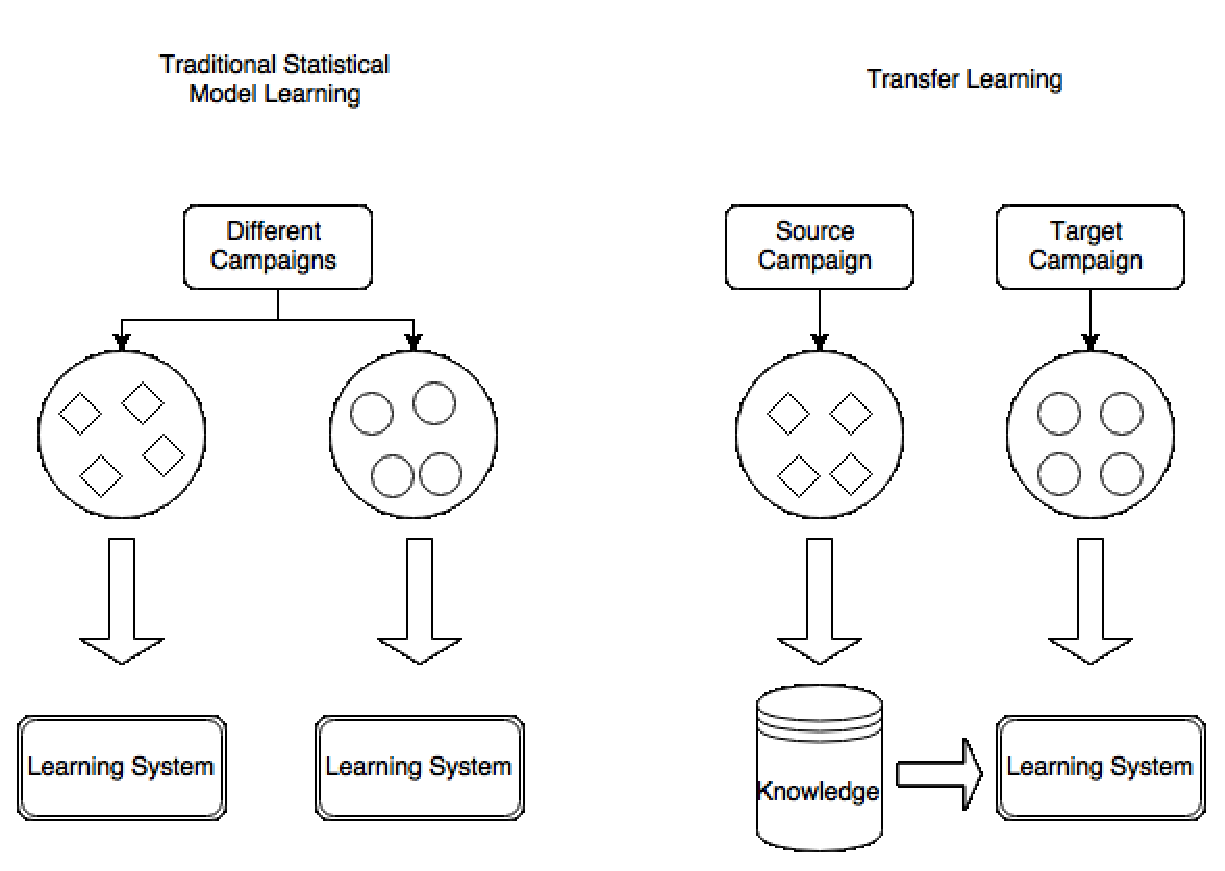
\includegraphics[width=\columnwidth]{transferlearning.eps}
\caption{Different Learning system between traditional machine learning and transfer learning}
\label{fig:transfer}
\end{figure}

At first, using the definitions in \cite{pan2010survey}, we specify \textit{domain} \textit{D} as each campaign's impressions raw data, and \textit{task} \textit{T} as the learning system of the model, in which, \(D = \{X,P(X)\}\), also  \(D = \{Y,P(Y|X)\}\). \(X = \{x_1,x_2, ..., x_n\}\) in which \(x_i\) is one impression in the campaign, and \(Y = \{y_1,y_2, ..., y_n\}\) is the label for each impression, namely whether in this impression the click occurs. The training data is composed of the pairs of \(\{x_i,y_i\}\) which can be used to train the model, and the conditional distribution \(P(Y|X)\). We define \textit{source domain} as the old campaign and \textit{target domain} as the new campaign, then \(X_s\) will be the feature space of source domain and \(P(X_s)\) is the marginal probability distribution of the feature space of source domain, similar, \(X_t\) will be the feature space of target domain and \(P(X_t)\) is the marginal probability distribution of the feature space of target domain. \(Y_s\) is the class label of the features in source domain and \(Y_t\) will be the corresponding label for target domain. By considering the relation between source domain and target domain, as well as source task and target task, the model learning problem can be classified as follows in the scope of online advertisement. 

\begin{enumerate}
\item if \(D_s = D_t\) and \(T_s = T_t\), this is a traditional machine learning problem. For example, the source and target advertisement campaigns follow the same distribution, and their learning tasks are the same, which are to predict the CTR based on the feature spaces. 

\item if  \(D_s \neq D_t\) and \(T_s = T_t\), which means the source and target domains are distinct but with the same tasks. The problem is also known as \textit{domain adaptation} \cite{arnold2007comparative} since the two domains are different in the marginal probability distribution but same for tasks. This situation can be further classified into two types:
    \begin{itemize}
    \item  \(X_s \neq X_t\), which means the feature spaces of the two domains are different with each other, for example, one domain of an advertisement campaign  \textit{International e-commerce} and the other is from \textit{ Software} as shown in \cite{zhang2014real}, if the impressions of the two domains are encoded into binary feature, surely there will be small overlap between the two feature spaces and the feature spaces will be largely different.
    \item \(P(X_s) \neq P(x_t) \), which means the probability distributions of the two advertisement campaigns are different, so they are from different fields, with different themes. 
    
    \end{itemize}
\item if  \(D_s = D_t\) and \(T_s \neq T_t\), it can also be classified into two types:
     \begin{itemize}
    \item  \(Y_s \neq Y_t\), this means the label spaces are different for two domains, as an example for online advertisement, the label in one domain could be click/non-click, which is dichotomic, but in the other domain the labels can be winning price, which is continuous.
    \item \(P(Y_s|X_s) \neq P(Y_t|X_t) \), this means the conditional probability distributions of the label on feature spaces are different for two domains, one example can be due to the existence of online robots, for one campaign all the impressions are randomly clicked or seen by programs, but the other campaign successfully prevent themselves from the robots so all clicks are effective and valid which simulates the human behaviors in the real world.  
  \end{itemize}
\end{enumerate}

In this paper, we will focus on transductive transfer learning, or \textit{domain adaptation}, since our learning task is obvious, which is CTR prediction, and we assumes that the robots are rare in the campaign, so the conditional probability are similar between the two campaigns, since the similar human behaviors will lead to similar advertisement clicking actions. 

As discussed above, domain is composed of feature space and feature probability distribution. In this paper, since our goal is to compare the performance of binary feature and counting feature, so we will represent the feature space and feature probability distribution of source and target domain in Table~\ref{tab:domainadapt}.

\begin{table}[t]
\begin{tabular}{ c | l | l }
Feature Types & Feature Space & Feature Distribution \\
\hline \hline
Binary Feature & Different & Different  \\
Counting Feature & Same & Different
\end{tabular}
\caption{Source and Target domain comparison for Binary and Counting Features}
\label{tab:domainadapt}
\end{table}

To clarify, for binary feature, suppose in the user dataset of online advertisement there is a categorical feature \textit{nationality}, with the value \textit{China}, \textit{Uk}, \textit{USA}, etc. It is not surprisingly that the original field space will be blew up to hundreds of features which is the number of countries in the world, without pre-processing, we even cannot distinguish \textit{Uk} from \textit{Great Britain}, which makes astronomical number of features with the increasing of new impressions. Microsoft claims that they have hundreds of millions features \cite{graepel2010web} for each training dataset, as we are already in the age of big data online advertisement, we can expect that the data volume will increase to the magnitude of hundred billion with hundred billion sparse discrete features. Even for our experiment, millions of features will arise from the dataset when the number of impressions reach 1 million. Therefore, the feature spaces are always distinct between the old campaigns and new campaigns. 









\subsection{Advertisement Campaign Datasets Shift}

\subsection{Cross-Dataset Generalization}



\section{Experiment}

\subsection{Experiment Setup, Dataset Introduction and Measurement Method}

In this part, the results of two experiments will be shown. At first, we will represent that the performance of counting feature on non-linear regression model is comparable to that of one-hot binary feature of linear regression model. Secondly, we will show that counting feature performs significantly better than binary feature in cross-domain learning problem. 

For Cross Domain problem, we will do the experiment in the following scenario. An ad company serves for different clients for CTR prediction. Based on the information from old campaigns, it hopes to get accurate CTR prediction result for new campaigns without training new model but directly make use the off-the-shelf model derived from old campaigns. \vspace{5mm}

In this experiment, the whole 14 days dataset will be splitted based on the client id so that in each sub dataset all impressions are from a unique client. To simulate the real world situation that the ad data is not static but performs as a continuous data stream, the new campaign dataset will be further divided into smaller data capsules. Then on the one side, the old campaign dataset will be transformed into binary feature dataset then the model will be trained based on it. Then capsules will be sent into the model in sequence to estimate its CTR thus AUC for test dataset will be obtained. \vspace{5mm}

While on the other side, counting feature bears the advantage that its number of features are limited, and feature values are continuous. So unlike 0-1 binary feature, it is possible to update the feature values as more information from new campaign arrives with fixed model weights. The representation of two scenarios can be represented as follows in Figure ~\ref{fig:binary} and Figure ~\ref{fig:counting}

\begin{figure}[t]
\centering
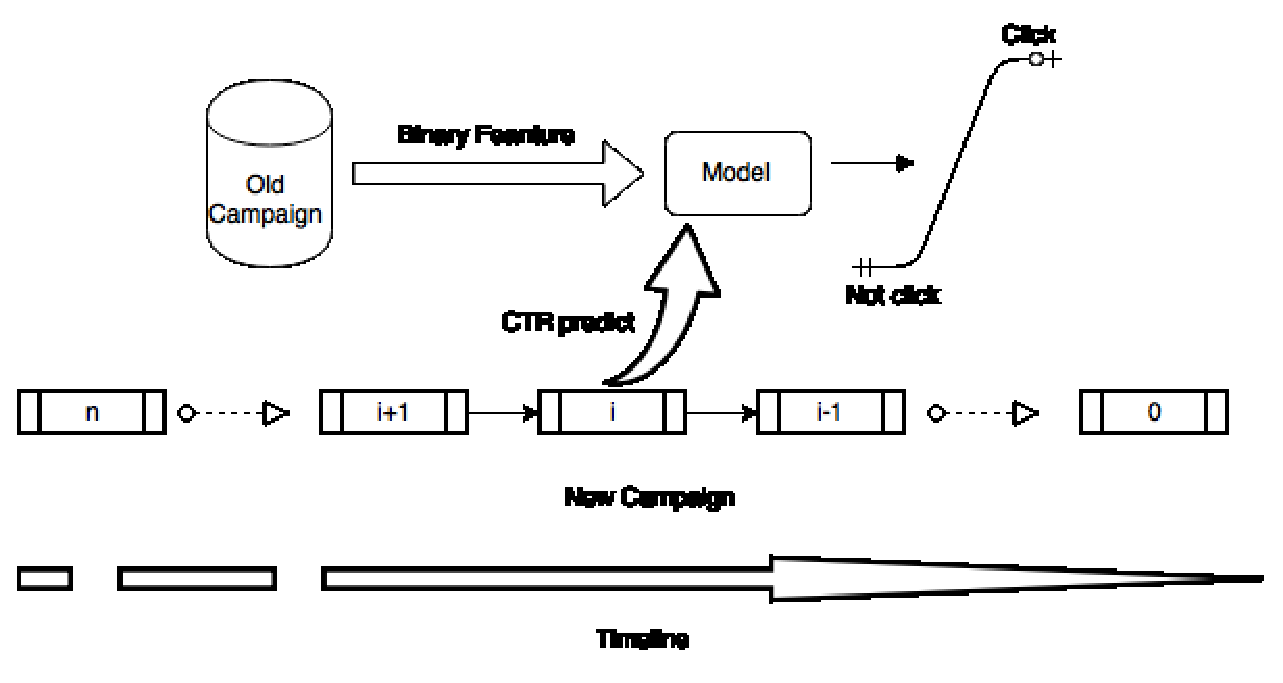
\includegraphics[width=\columnwidth]{binaryrepresent.eps}
\caption{Estimate new campaign CTR using Binary Feature}
\label{fig:binary}
\end{figure}

\begin{figure}[h]
\centering
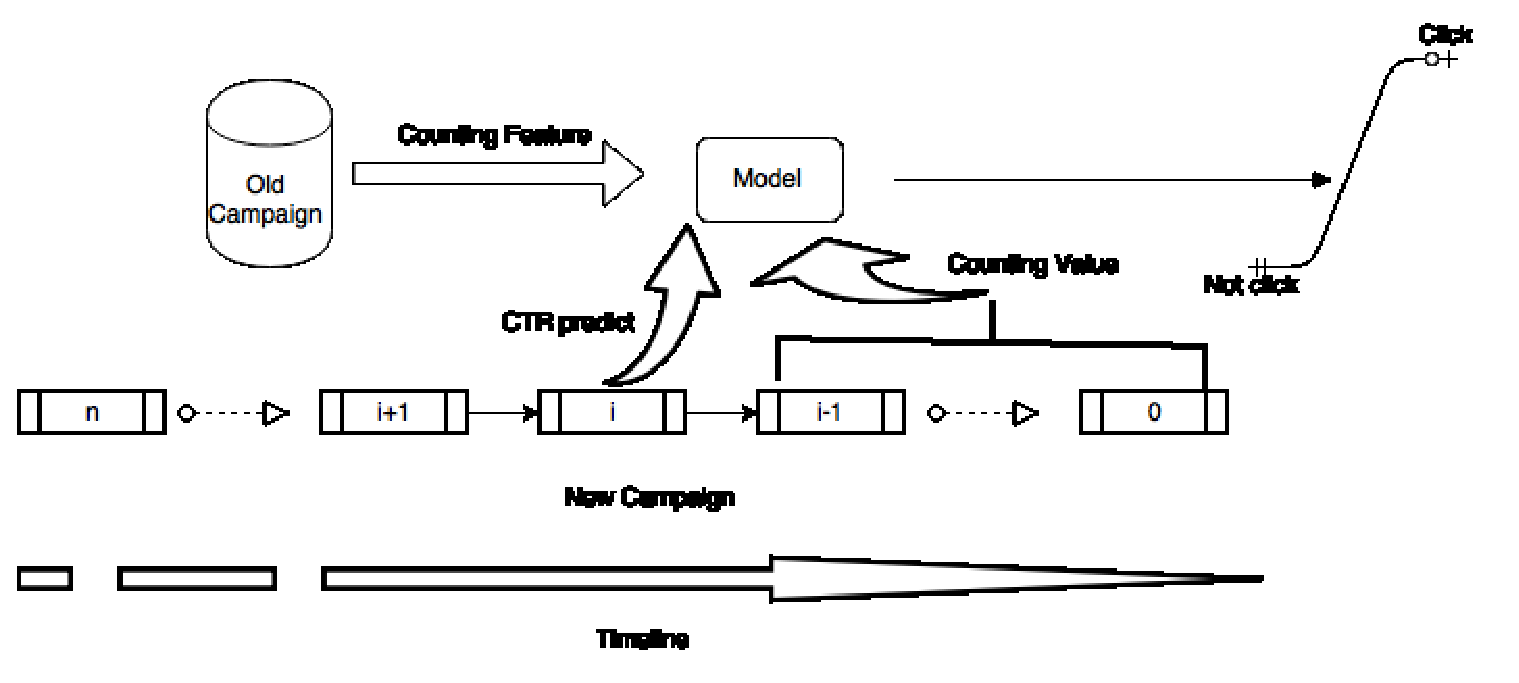
\includegraphics[width=\columnwidth]{counting.eps}
\caption{Estimate new campaign CTR using Counting Feature}
\label{fig:counting}
\end{figure}


\subsection{Performance Comparison of Binary and Counting Feature in CTR prediction Problem}

In this section two experiments are conducted to compare the CTR prediction performance of Binary and Counting feature in terms of logistic regression and gradient boosting regression tree (GBRT) model. The first experiment is based on the public dataset from Ipinyou, which was released by the Chinese RTB company Ipinyou for global RTB algorithm competition in 2013. The dataset includes logs of ad auctions, bids, impressions, and also clicks \ref{zhang2014real}. All the features except for \textit{Usertag} are used in the experiment due to the bias in that feature. The result is as follows:





\begin{figure}[h]
\centering
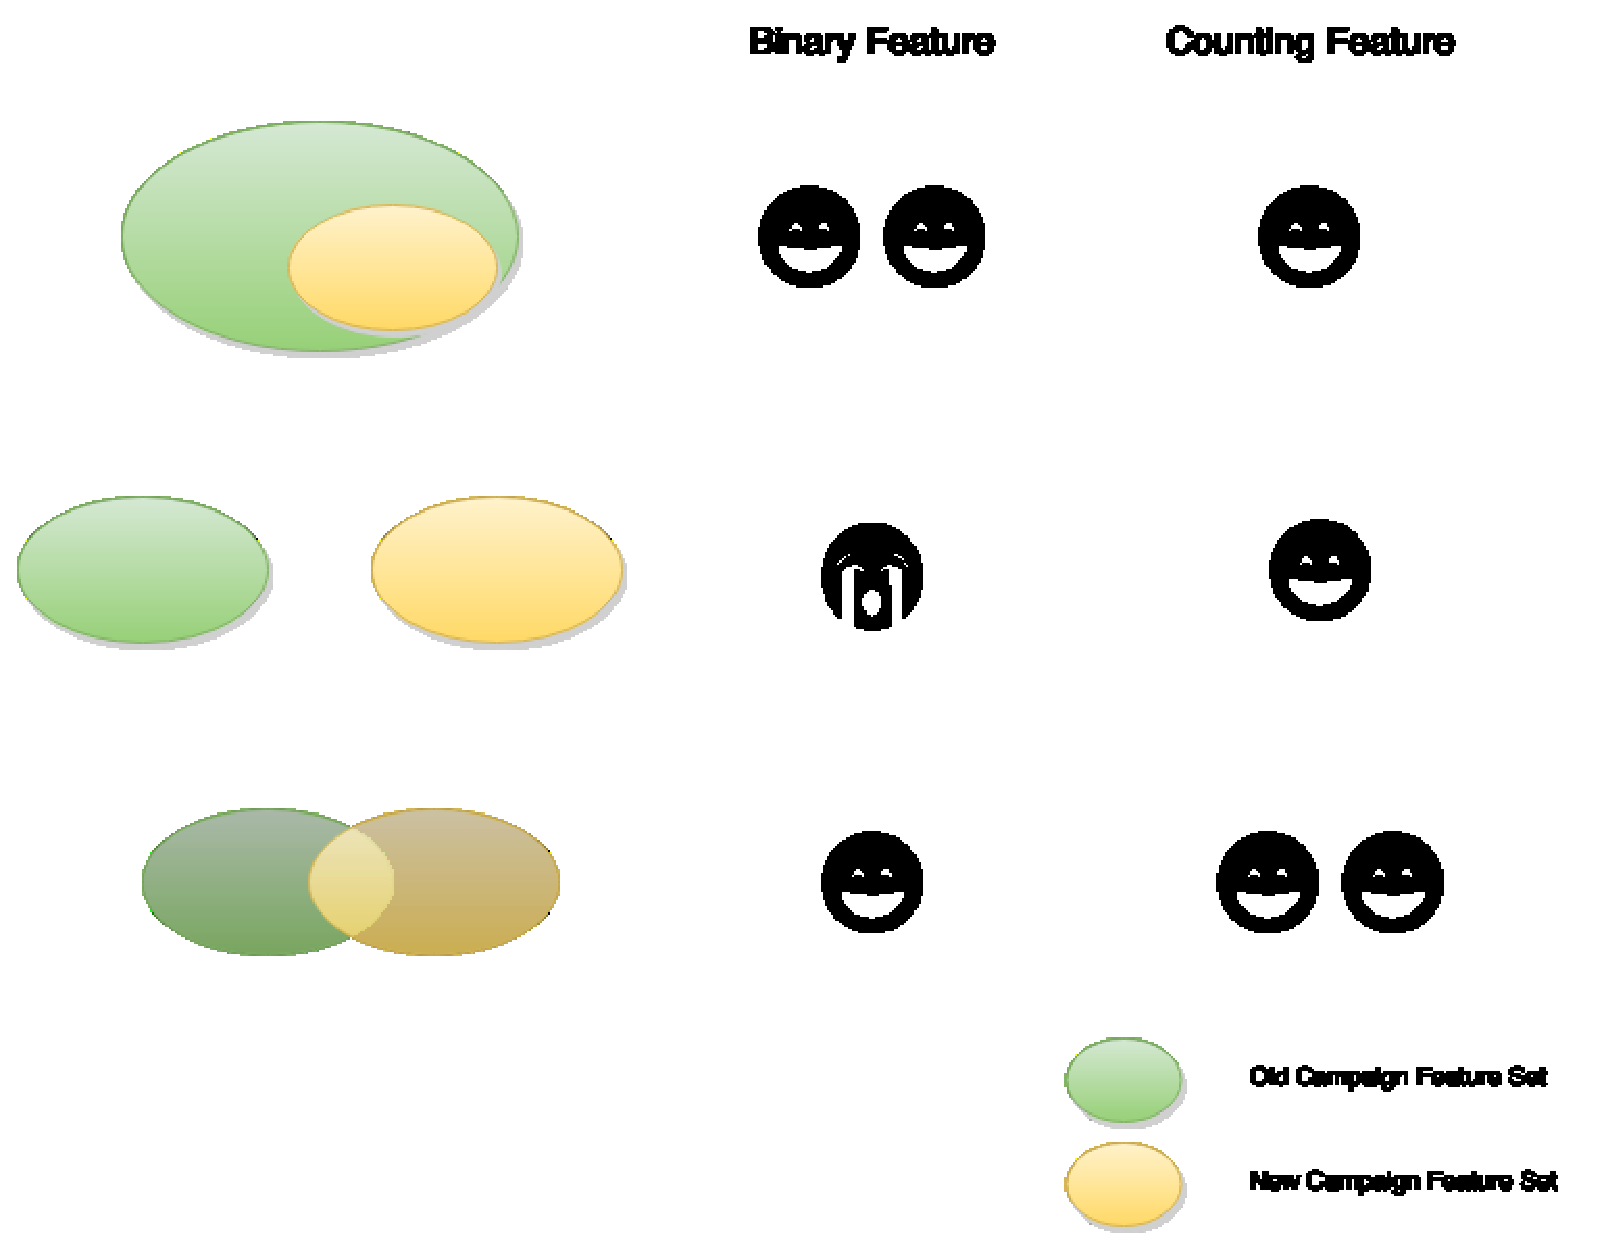
\includegraphics[width=\columnwidth]{Datasetbias.eps}
\caption{Three types of relation of feature sets between train dataset and test dataset}
\label{fig:datasetbias}
\end{figure}

\subsection{Performance Comparison of Binary and Counting Feature in Cold Start Problem}

In this part, the experiments will be done based on the dataset provided by a ad company in March which includes the data for 14 consecutive days, the dataset are separated by client id so that in each small dataset there are only the impressions from one unique client. In this experiment, the client with more than 500,000 impression are chosen so that 4 sub datasets are obtained which are from distinct clients. The detail of the four clients are shown in Table~\ref{tab:campainid}.


\begin{table}[t]
\centering
\begin{tabular}{c | c | c | c }
· 
\end{tabular}
\caption{Statistical Information of top 10 advertisement clients}
\label{tab:campainid}
\end{table}

\iffalse
\begin{table}[t]
 \centering
 \begin{tabular}{ ||c c || } 
 \hline
 Client id  & Number \\
 \hline
 20762 & 1068606 \\ 
  15140 & 764355 \\ 
   1371 & 576709 \\ 
   12482 & 557120\\
 \hline
 \end{tabular}
 \caption{Four Biggest clients}
 \label{tab:campainid}
 \end{table}
 
\fi

The figure above shows the truth that dataset significantly decide upper bound of the accuracy to predict CTR. above performance comparison of binary feature and counting feature on CTR estimation reveals that performance of counting feature using non-linear regression model is comparable to that of binary feature using linear regression model, the precondition is that the training and test dataset share most of the features. However, in real world we will always be faced up with the situation that the information is unbalanced in train and test dataset. We define \textit{Feature Set} as a criterion to measure the information obtained in the dataset, which is represented by  \(S_i(f)\), in which \(f\) are the unique features in the dataset \(i\).\vspace{5mm}

The relation of the feature sets in dataset \(i\) and \(j\) can be catogrized into three types, in which \(i\) is the test dataset, and \(j\) is the training dataset, as shown in Figure~\ref{fig:datasetbias}.:
\begin{itemize}
\item When \(s_i \subset s_j\), the binary feature should perform better than counting feature in terms of CTR estimation. Since in this way all the feature information needed by test dataset is inclusive in training dataset, the model contains all the infomraiton as a general model, as with the above conclusion when both using linear logistic regression, binary feature is superior to counting feature.  
\item When \(s_i \cap s_j \equiv 0\), the counting feature should perform better than binary feature which degenerates into random algorithm. The reason is that there is no overlap between \(s_i\) and \(s_j)\), so all feature information in test dataset will be regared as \textit{other} for model derived from training dataset. However, for counting feature, this deficiency can be made up with the gradual increasing information of the dataset distribution. The counting value to some extent represents the feature distribution so when we assume that the train and test dataset share similar feature value distribution counting feature can still perform rather well while at same time prediction using binary feature is totoally impossible.
\item When \(s_i \cap s_j \neq 0\), the feature informaiton at this time is shared by train and test dataset. We define \textit{General Information} as the information shared by all the advertisement campaigns, and \textit{Specific Information} as the unique feature information owned by each of the campaign. In this situation, both binary feature and counting feature performs well granted that train and test dataset share enough feature information so that the model to some extent is universal among datasets. However, the upper-bound of performance of binary feature is around the AUC result of the CTR prediction for first data capsule in the data stream assuming the distribution among test dataset is identical, conversely, that is the lower-bound of the performance of counting feature since with the increasing of test instances, counting value will tend towards the real distribution of test dataset to compensate of the unbalanced counting weights value. 
\end{itemize}



\begin{figure}[t]
\centering
\includegraphics[width=\columnwidth]{coldstart_first.eps}
\caption{Performance Comparison of Binary and Counting feature for Cross Domain Learning before Counting Value Updating}
\label{fig:coldstart_first}
\end{figure}

\begin{figure}[t]
\centering
\includegraphics[width=\columnwidth]{coldstart.eps}
\caption{Performance Comparison of Binary and Counting feature for Cross Domain Learning after convergence}
\label{fig:coldstart}
\end{figure}

\begin{figure}[t]
\centering
\includegraphics[width=\columnwidth]{coldstartimprove.eps}
\caption{Performance Comparison of Binary and Counting feature for Cross Domain Learning after convergence}
\label{fig:coldstartimprove}
\end{figure}

Figure \ref{fig:coldstart_first} shows the comparison of the performance between binary feature and counting feature before updating counting values. As shown in the diagram above, for binary feature the counting value will be updated between 0 and 1 since it is discrete, however, because the values of counting feature is continuous, so it is possible to update its values with the introduction of new data from new campaign. Figure \ref{fig:coldstart_first} shows the fact that just after training the model from old campaign, directly using it to predict the CTR of new campaign, binary and counting features are suffering from the same bad performance. 

Figure \ref{fig:coldstart} shows the fact that counting feature indeed improve the performance of CTR prediction after a few times updating until convergence. After getting information from the new coming data, the counting value will be changed to represent the distribution of the new campaign somehow, which takes over the responsibility from the binary weights space. However for binary feature since its feature space is fixed so changing between 0 and 1 cannot represent the distribution of the new campaign so there is no performance improvement for binary feature after the updating. 

Figure \ref{fig:coldstartimprove} demonstrates the conclusion in last above well. If we assume that the distribution of the new campaign is identical, the performance of the CTR prediction in terms of AUC should be the same among all sub-dataset of the new campaign. We define  \(AUC_{\text{before}}\) as the CTR prediction performance for the first capsule of new campaign data, when there is no counting value update from new campaign and we can only predict it based on the model from the old campaign. We also define \(AUC_{\text{after}}\) as the peformance of binary or counting feature after all the information of the new campaign has been obtained by the model and it becomes converged. In Figure \ref{fig:coldstartimprove} we compare the\({AUC_{\text{after}}}/{AUC_{\text{before}}}\)
for binary feature and counting feature.From the plot it shows that for binary feature there is no improvement for most cases since the value is around 1 and for counting feature the improvement is high. 



Figure \ref{fig:matrixbefore} \ref{fig:matrixafter} and \ref{fig:matriximprove} shows the details of the result.In Figure \ref{fig:matrixbefore} we calculate \((AUC_{\text{before(count)}} - AUC_{\text{before(bi)}}) / AUC_{\text{before(bi)}} \) to show how counting feature improves the performance compared to binary feature before updating the counting values, the result shows that counting feature performs bad which is not surprising. 

In Figure \ref{fig:matrixafter} we shows the same calculating for that but after updating the counting values.  \((AUC_{\text{after(count)}} - AUC_{\text{after(bi)}}) / AUC_{\text{after(bi)}} \) is shown in the matrix. Green shows that the counting feature performs better than binary feature, and the percentage value shows by how many percents do the counting feature obtains in terms of CTR AUC performance. It shows that excluding the diagonal in which the train and test dataset are the same, so the binary feature should perform better than counting feature, In 61 out of 90 experiments counting feature performs better than binary feature, which is much better than we can see in Matrix \ref{fig:matrixbefore}.

Figure \ref{fig:matriximprove} calculates 
\((AUC_{\text{after(count)}}/AUC_{\text{before(count)}} -AUC_{\text{after(bi)}}/AUC_{\text{before(bi)}})  / (AUC_{\text{after(bi)}}/AUC_{\text{before(bi)}})  \), which shows that after updating the counting value, whether counting feature gains more performance improvement than binary feature, result shows that counting feature indeed improves much more than binary feature whose upper bound of CTR estimation is decided when the first subset of data comes. 

\begin{figure}[t]
\centering
\includegraphics[width=\columnwidth]{matrixbefore.eps}
\caption{Percentage of Performance Improvement of Counting Feature to Binary Feature in Cross Domain Learning before Counting Value Updating}
\label{fig:matrixbefore}
\end{figure}

\begin{figure}[t]
\centering
\includegraphics[width=\columnwidth]{matrixafter.eps}
\caption{Percentage of Performance Improvement of Counting Feature to Binary Feature in Cross Domain Learning After Convergence}
\label{fig:matrixafter}
\end{figure}

\begin{figure}[t]
\centering
\includegraphics[width=\columnwidth]{matriximprove.eps}
\caption{Percentage of Performance Improvement of Counting Feature Compared to Binary Feature}
\label{fig:matriximprove}
\end{figure}


\begin{figure}[t]
\centering
\includegraphics[width=\columnwidth]{variance.eps}
\caption{Cross-validation of binary and counting feature dataset mean and variance}
\label{fig:variance}
\end{figure}

\begin{figure}[t]
\centering
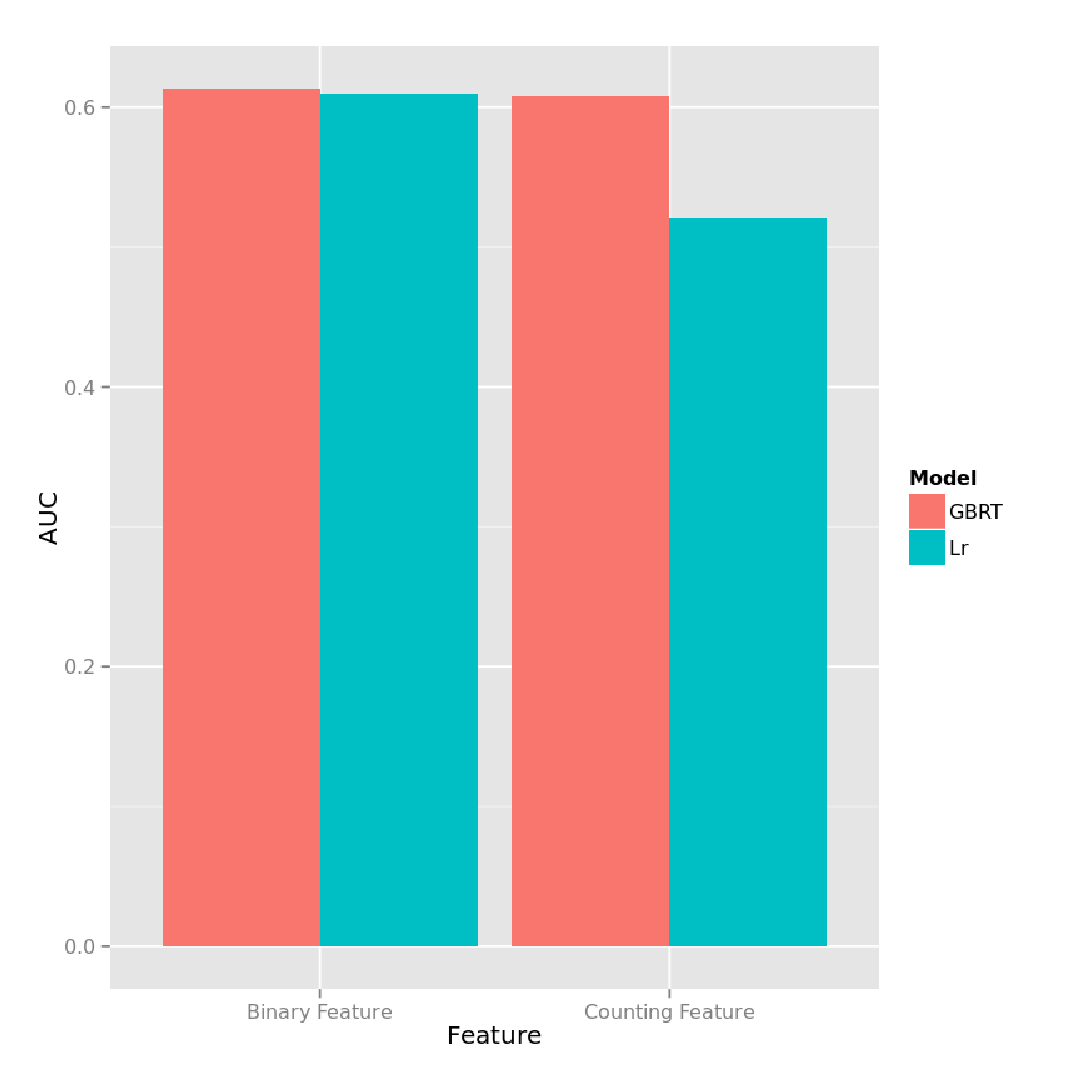
\includegraphics[width=\columnwidth]{2261.eps}
\caption{Performance 2261}
\label{fig:2261}
\end{figure}

\begin{figure}[t]
\centering
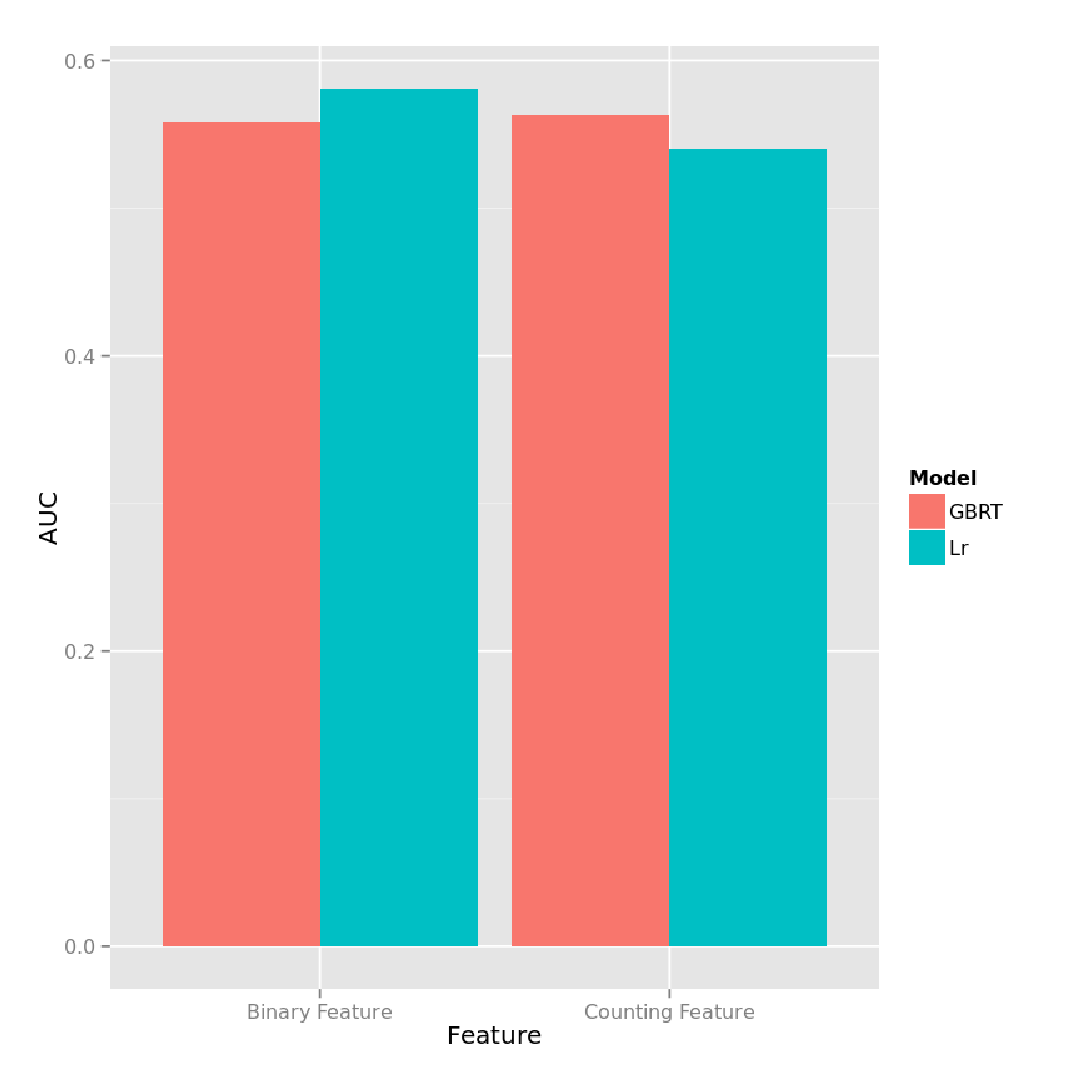
\includegraphics[width=\columnwidth]{2997.eps}
\caption{Performance 2997}
\label{fig:2997}
\end{figure}

\begin{figure}[t]
\centering
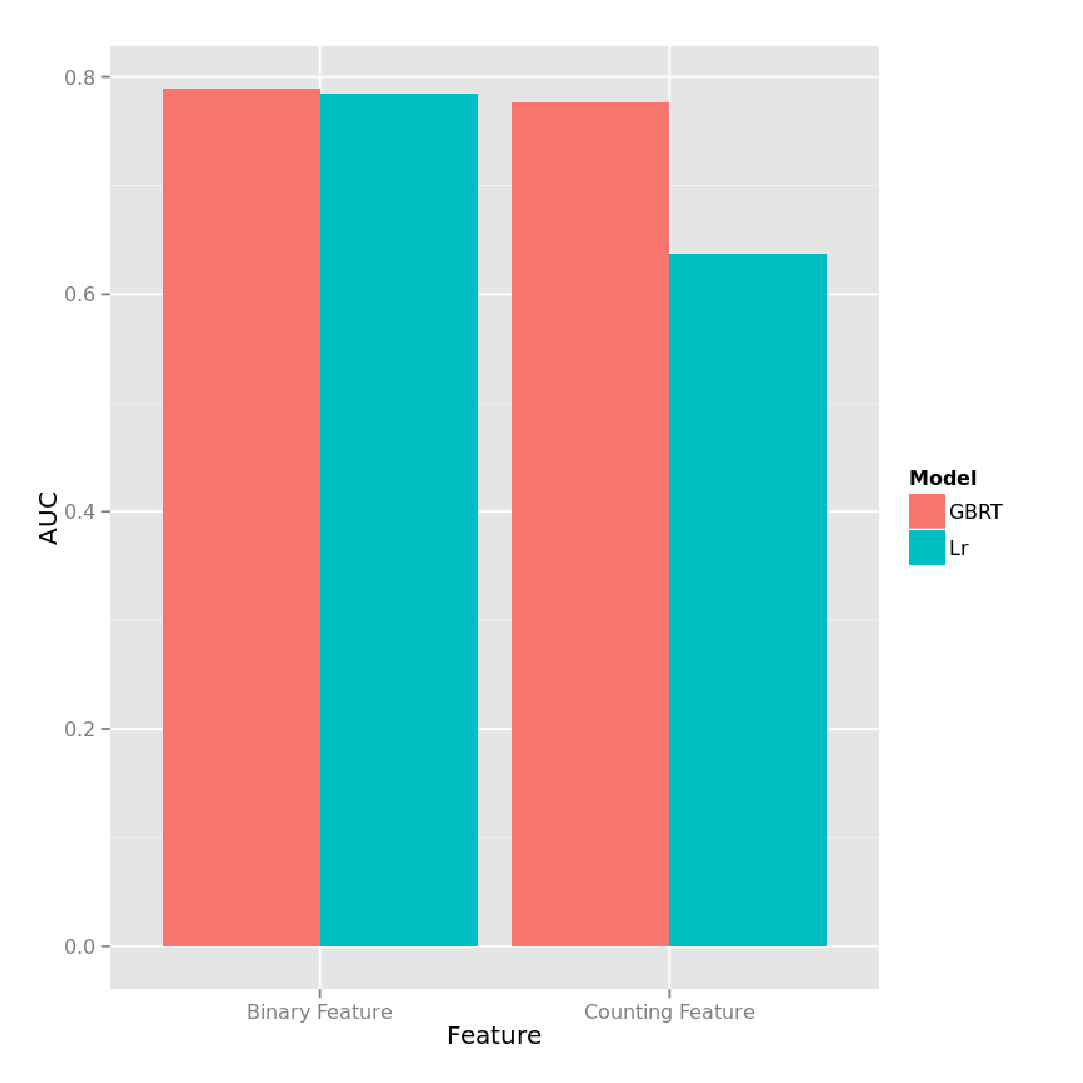
\includegraphics[width=\columnwidth]{3386.eps}
\caption{Performance 3386}
\label{fig:3386}
\end{figure}


% The data from 3-14 to 3-27 are regarded as training dataset, the data from 5- are regarded as test dataset, the count of training dataset is, test dataset is ~\ref{tab:campainid}

% \begin{table*}[h]
% \centering
% \begin{tabular}{ |c|c|c|c| } 
% \hline
% Shared Campaign  & Unique Train Dataset Campaign & Unique Test Dataset Campaign \\
% \hline
% 1310190 & 1307617, 884194, 1283235, 1335301  & 1466432, 1448738 \\ 
% & 1385319, 1349577, 1276074, 1363723 & 1406405, 1424966 \\ 
% &  1357245, 1341802, 1341937, 1307838 & 1424330, 1445998 \\ 
% &  1285558, 1358167, 1305663, 1299899 & 1458704, 1454382 \\
% &  1363711, 1386205, 1368830, 1366271 &  1472727, 1452138 \\
% \hline
% \end{tabular}
% \label{tab:campainid}
% \end{table}

% Only the instances from the campaign with more than 500 clicks and 50000 impressions will be remained, the campaigns can be classified as the ones shared by the training and test dataset, the ones unique to training dataset and the one unique to test dataset.  

% \(1/3\) of the training dataset is used as train dataset, \(2/3\) will be used as count dataset. In order to increase the generalization of training dataset to improve the universality of the trained prediction model, four campaign will constitute one training dataset and two campaigns are used to make up a test dataset to decrease the bias of test dataset.  

% For the sake of convenience, the training dataset will be labeled as 1,2,3,4 and 5, from top to the bottom, as well as the test dataset. For each training dataset, the prediction model will be build based on it which will be used to test the data stream from each of the test dataset, the result is in 6.3.


\begin{figure*}
    \centering
    \begin{subfigure}[b]{0.3\textwidth}
        \centering
        \includegraphics[width=\textwidth]{cos}
        \caption{Cos Similarity Comparison Between Pairwise of Binary Feature and Counting Feature}
        \label{fig:cos}
    \end{subfigure}
    \hfill
    \begin{subfigure}[b]{0.3\textwidth}
        \centering
        \includegraphics[width=\textwidth]{correlation}
        \caption{Correlation Similarity Comparison Between Pairwise of Binary Feature and Counting Feature}
        \label{fig:correlation}
    \end{subfigure}
    \hfill
    \begin{subfigure}[b]{0.3\textwidth}
        \centering
        \includegraphics[width=\textwidth]{euclidean}
        \caption{Euclidean Distance Comparison Between Pairwise of Binary Feature and Counting Feature}
        \label{fig:euclidean}
    \end{subfigure}
    \caption{Comparison of Binary and Counting Feature Model Weights Space}
    \label{fig:three graphs}
\end{figure*}


Figure \ref{fig:variance} shows that the variance and mean for binary and counting feature dataset are nearly the same. 

Figure \ref{fig:three graphs} shows that the similarity among weights space for counting feature is higher than counting feature. 



\iffalse
Experiment 1.1: Training Dataset  (20762), Test Dataset  (15140) in Figure~\ref{fig:fig1}.:
\begin{figure}[h]
\centering
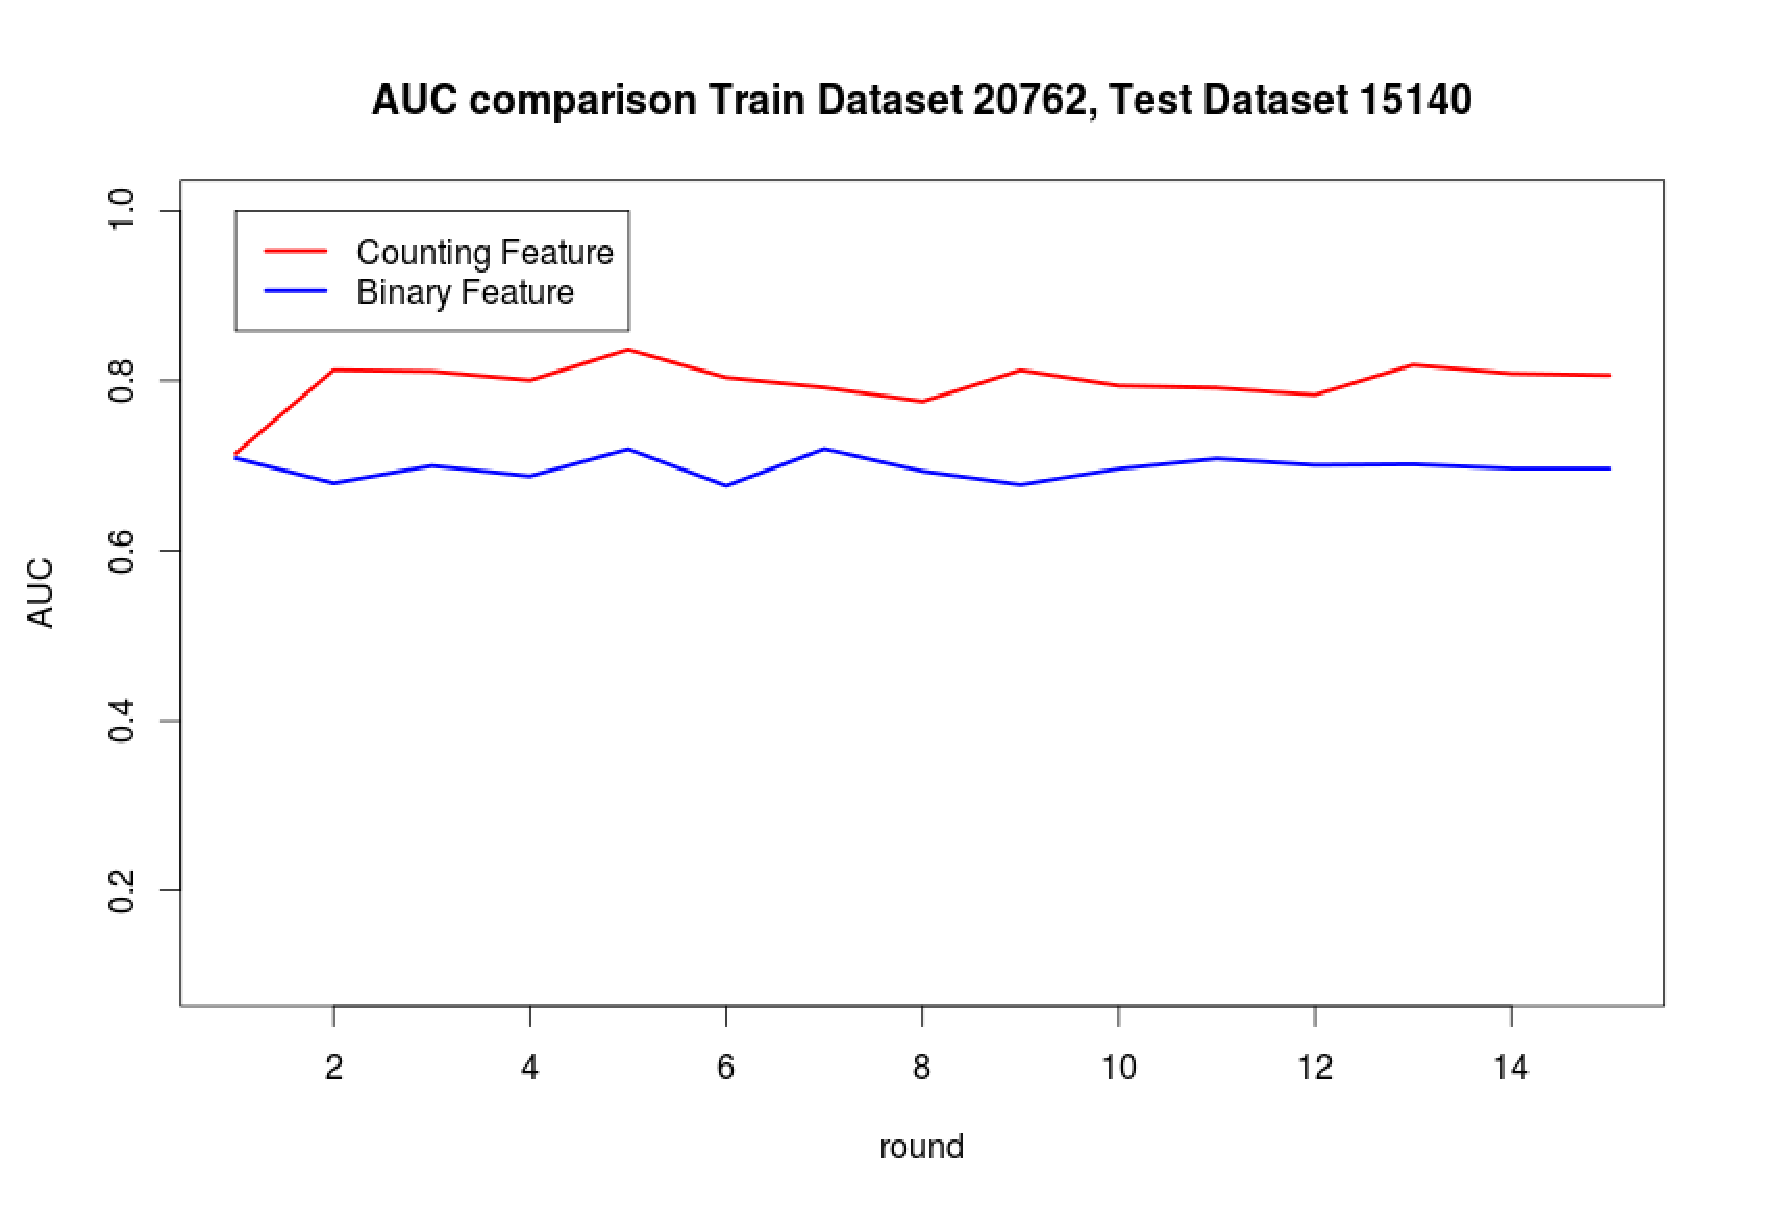
\includegraphics[width=\columnwidth]{20762_15140.eps}
\caption{Training Dataset  (20762), Test Dataset  (15140)}
\label{fig:fig1}
\end{figure}

Experiment 1.2: Training Dataset  (20762), Test Dataset  (1371) in Figure~\ref{fig:fig2}.:
\begin{figure}[h]
\centering
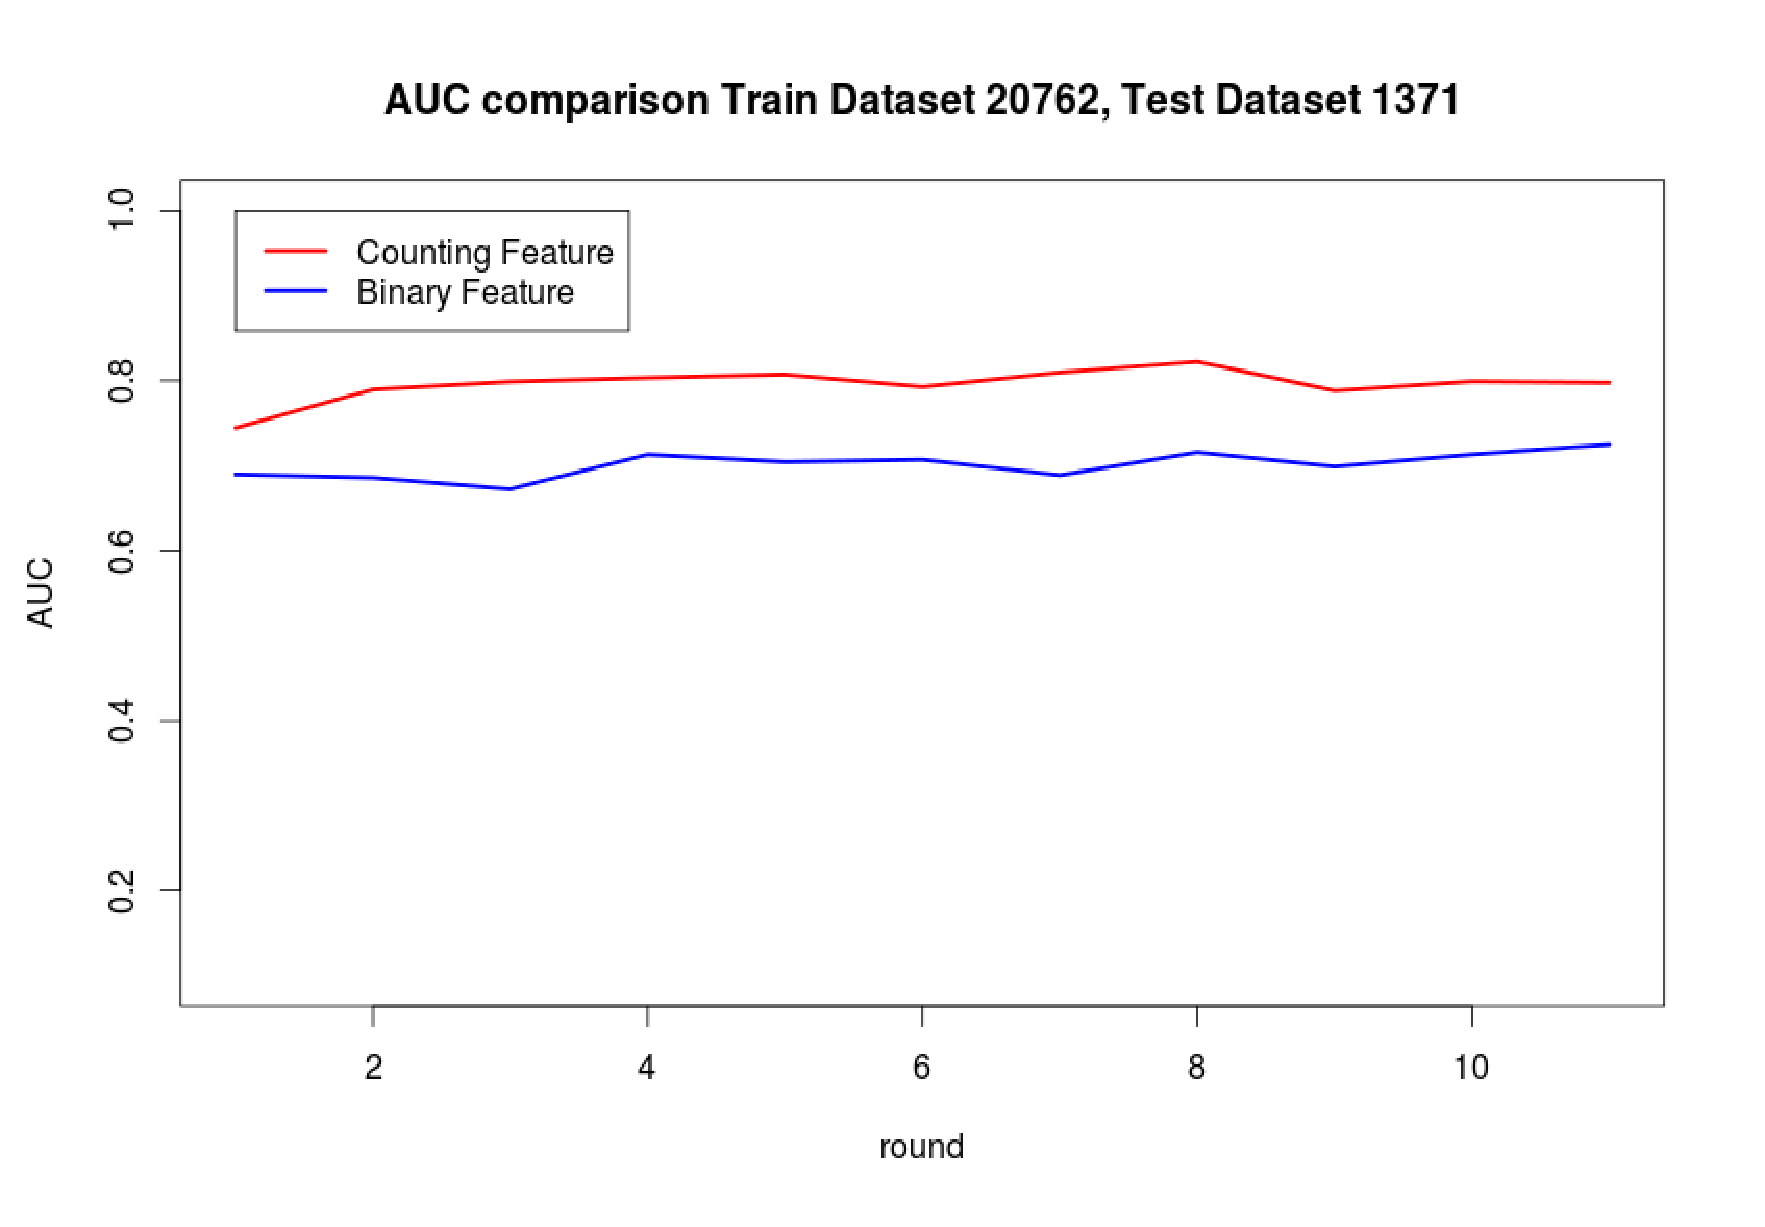
\includegraphics[width=\columnwidth]{20762_1371.eps}
\caption{Training Dataset  (20762), Test Dataset  (1371)}
\label{fig:fig2}
\end{figure}

Experiment 1.3: Training Dataset  (20762), Test Dataset  (12482) in Figure~\ref{fig:fig2}.:
\begin{figure}[h]
\centering
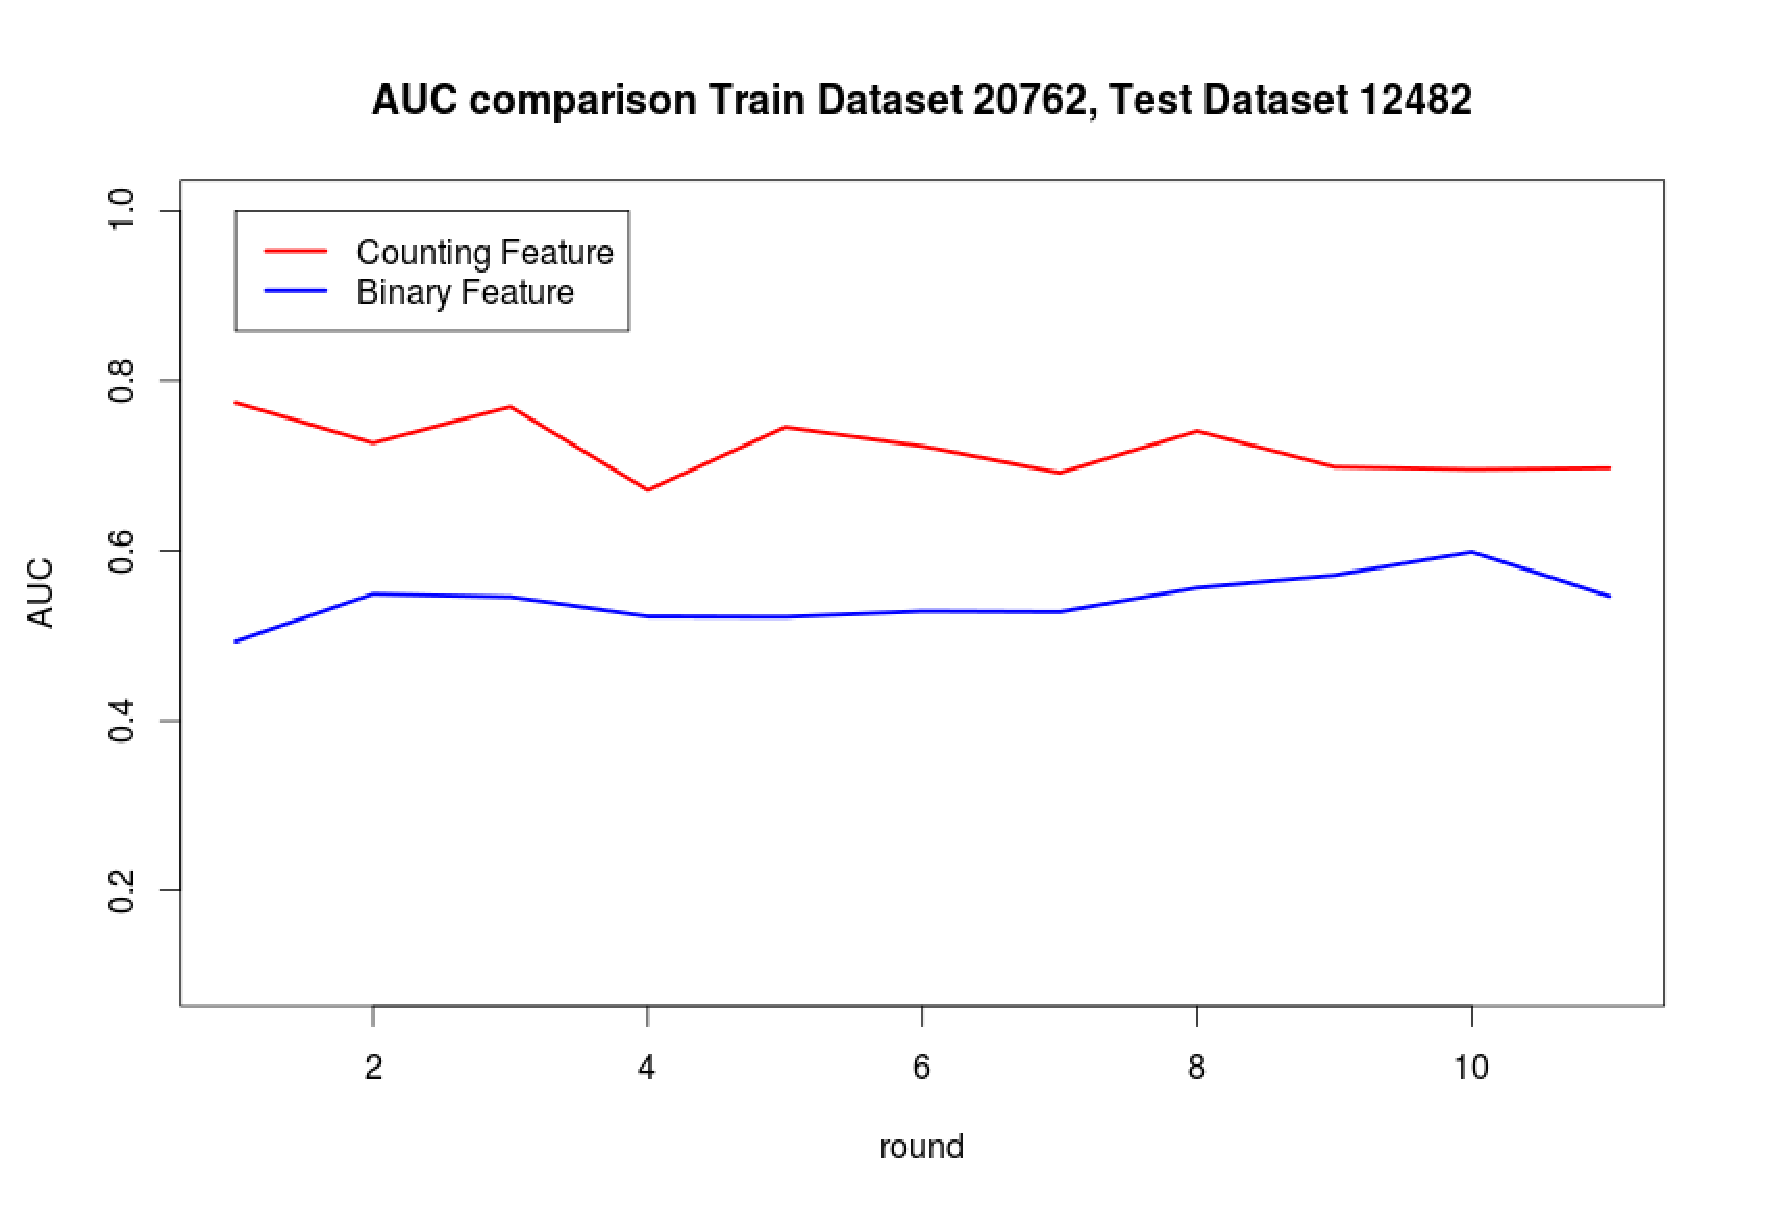
\includegraphics[width=\columnwidth]{20762_12482.eps}
\caption{ Training Dataset  (20762), Test Dataset  (12482)}
\label{fig:fig2}
\end{figure}

Experiment 2.1: Training Dataset  (15140), Test Dataset  (20762) in Figure~\ref{fig:fig3}.:
\begin{figure}[h]
\centering
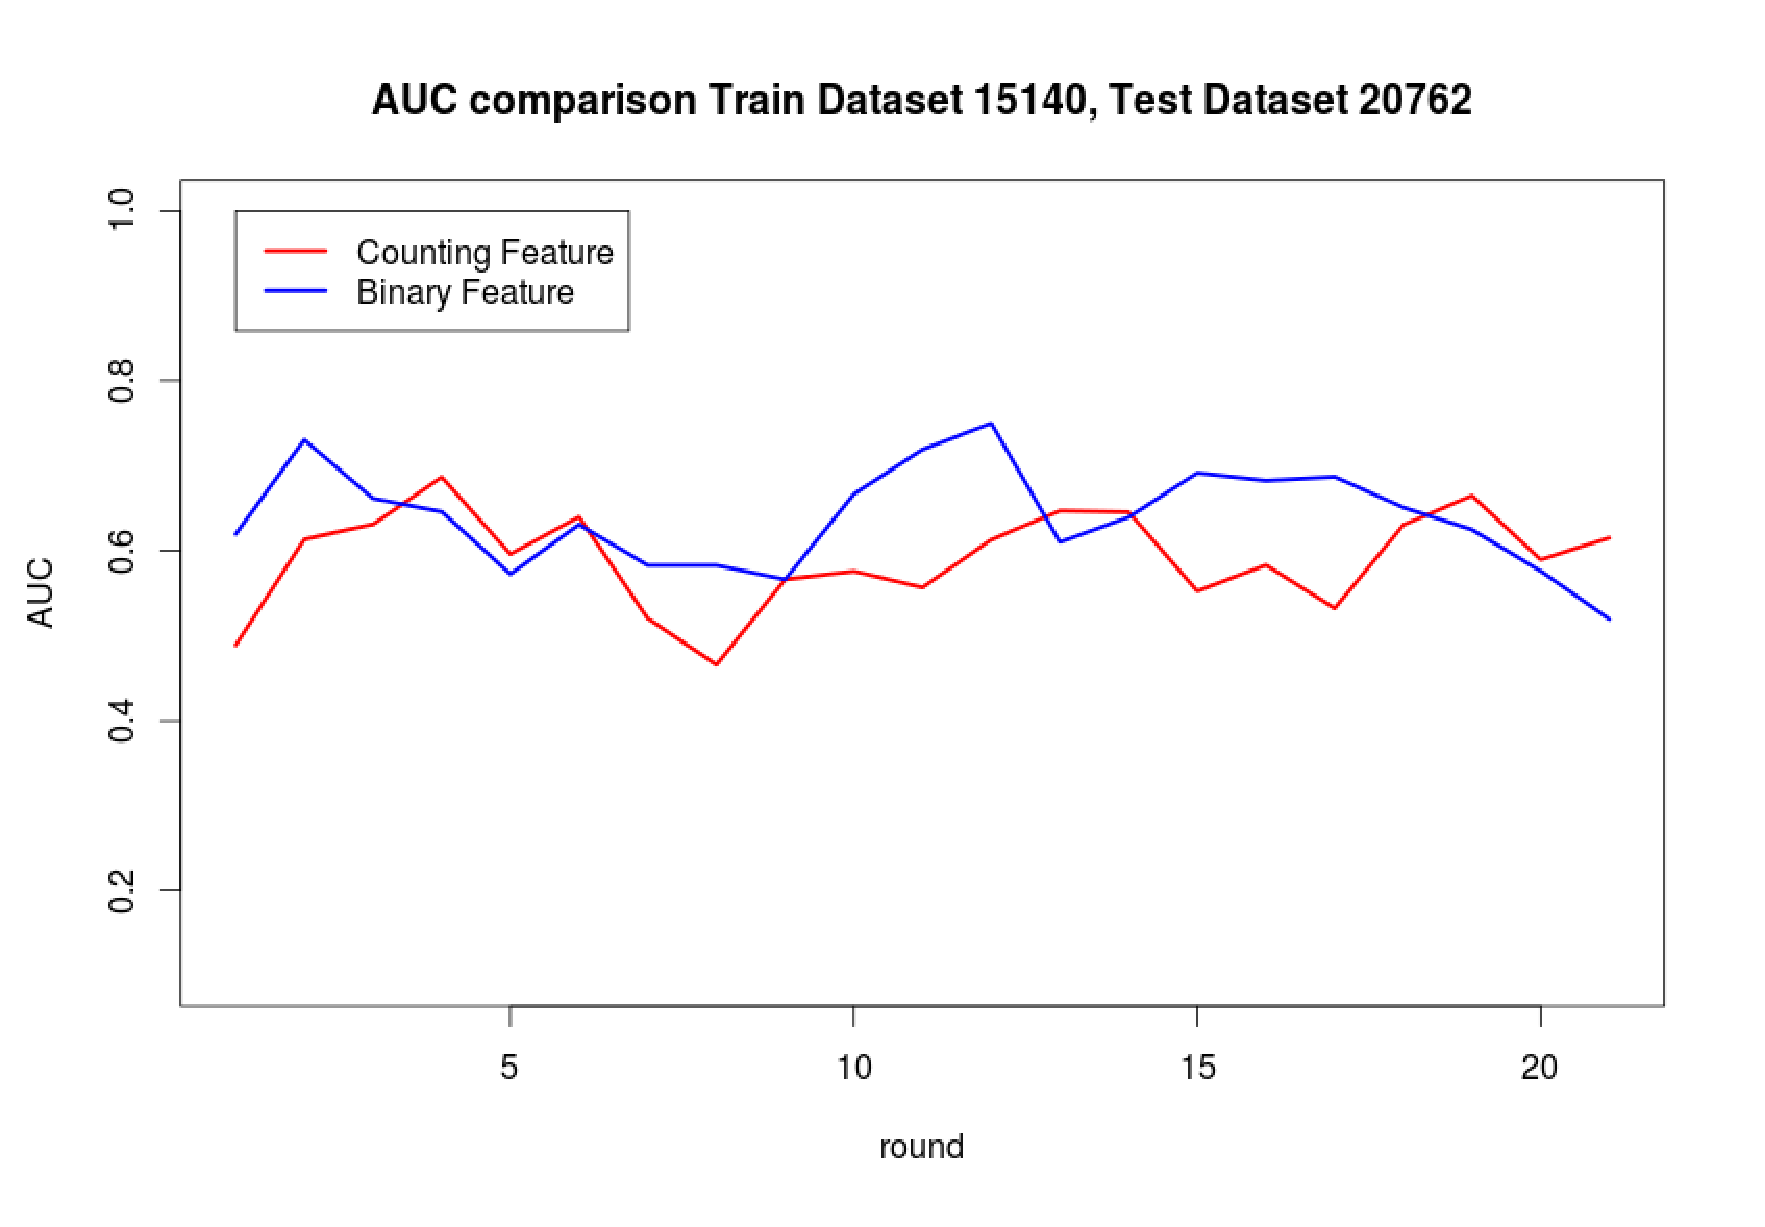
\includegraphics[width=\columnwidth]{15140_20762.eps}
\caption{Training Dataset  (15140), Test Dataset  (20762)}
\label{fig:fig3}
\end{figure}

Experiment 2.2: Training Dataset  (15140), Test Dataset  (1371) in Figure~\ref{fig:fig4}.:
\begin{figure}[h]
\centering
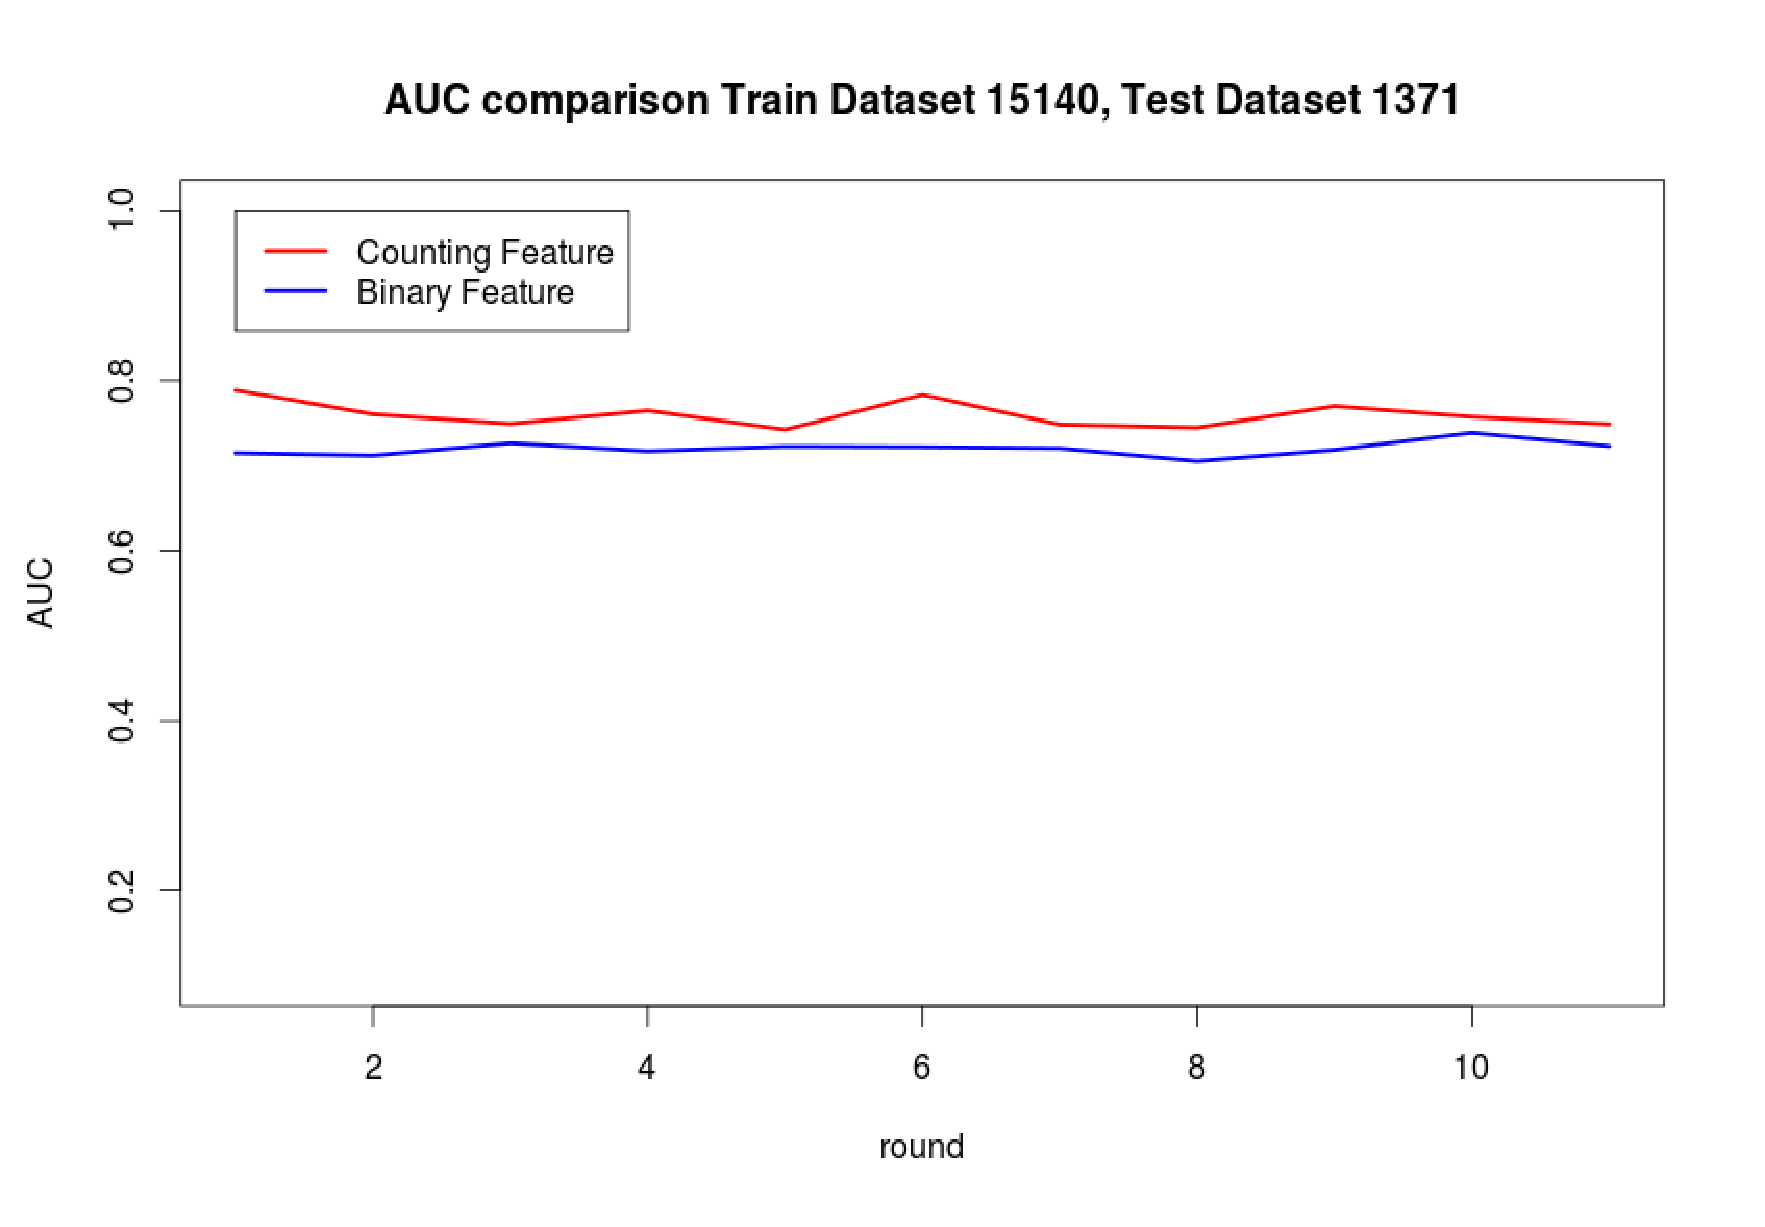
\includegraphics[width=\columnwidth]{15140_1371.eps}
\caption{Training Dataset  (15140), Test Dataset  (1371)}
\label{fig:fig4}
\end{figure}

Experiment 2.3: Training Dataset  (15140), Test Dataset  (12482) in Figure~\ref{fig:fig5}.:
\begin{figure}[h]
\centering
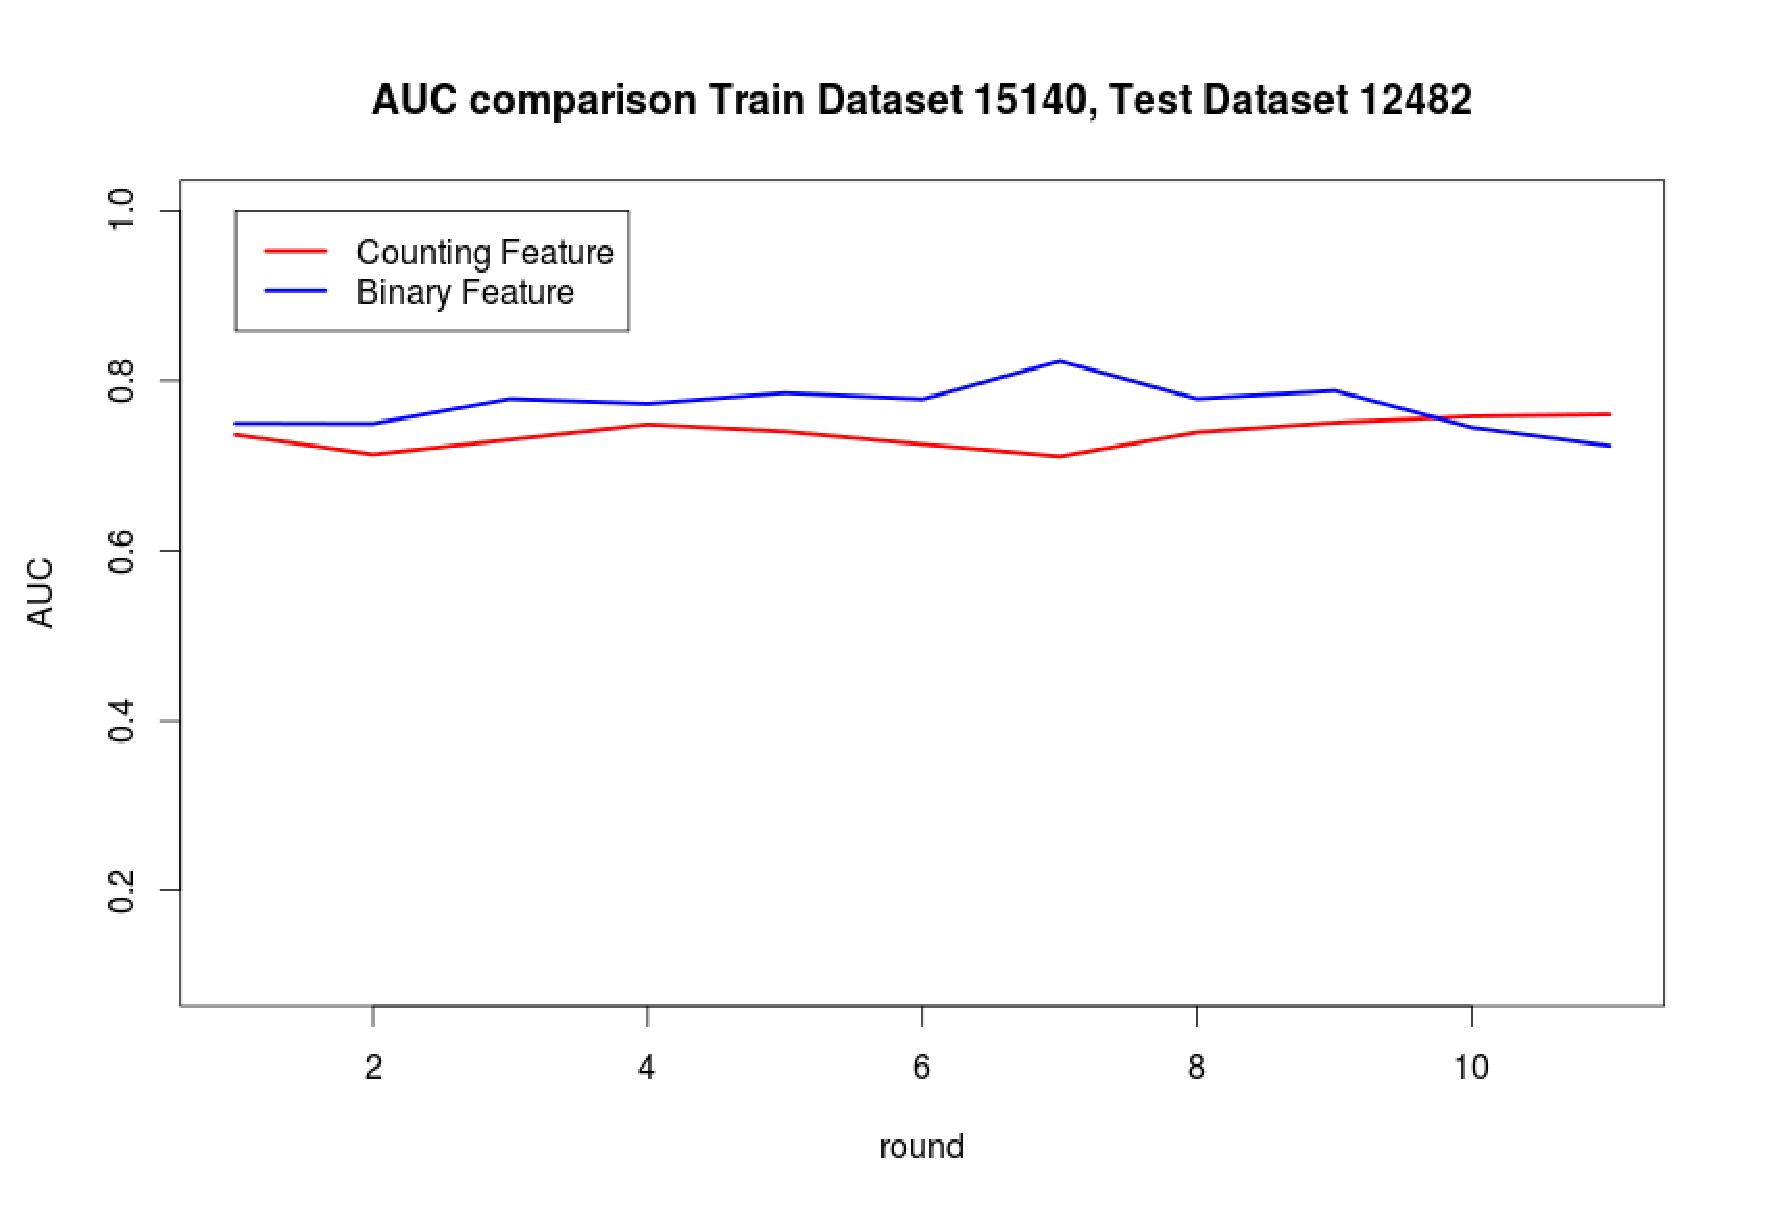
\includegraphics[width=\columnwidth]{15140_12482.eps}
\caption{Training Dataset  (15140), Test Dataset  (12482) }
\label{fig:fig5}
\end{figure}

Experiment 3.1: Training Dataset  (1371), Test Dataset  (20762) in Figure~\ref{fig:fig6}.:
\begin{figure}[h]
\centering
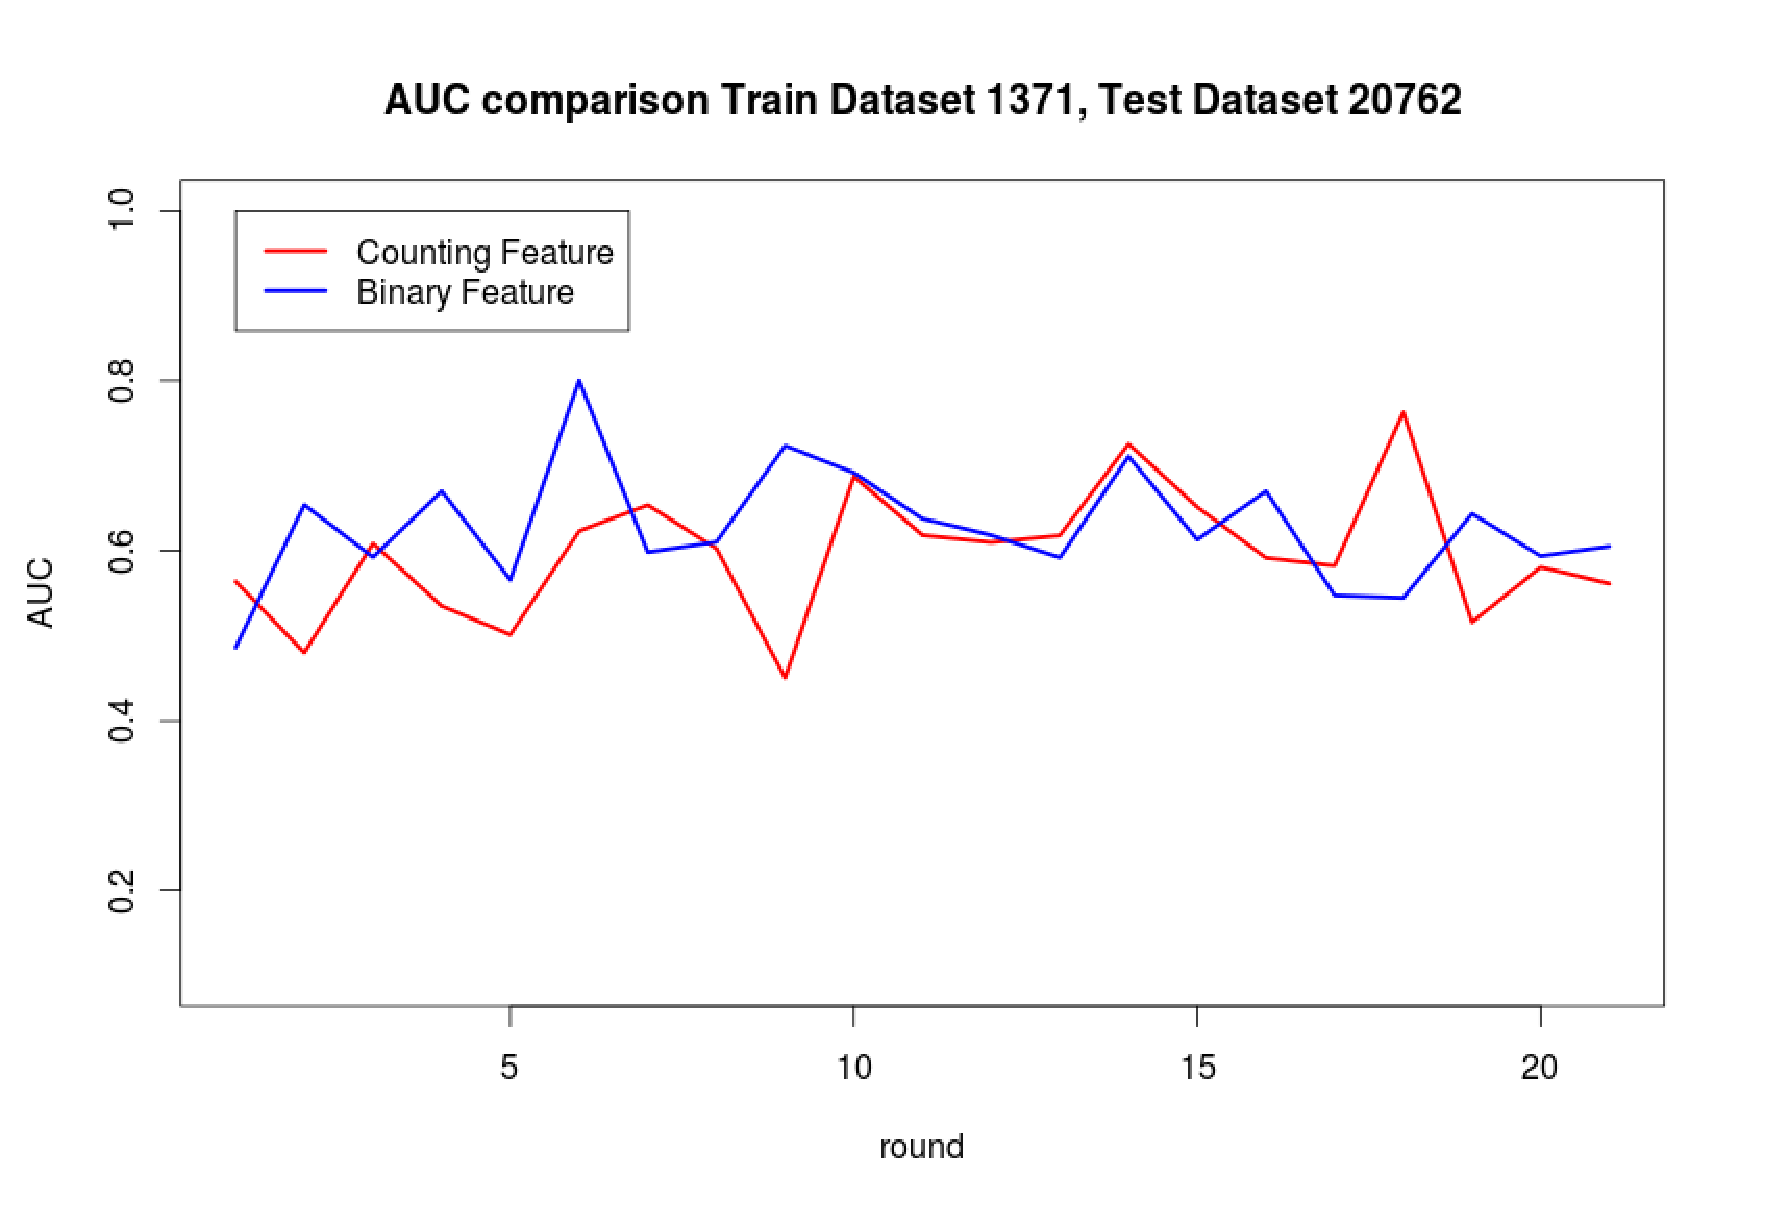
\includegraphics[width=\columnwidth]{1371_20762.eps}
\caption{ Training Dataset  (1371), Test Dataset  (20762)}
\label{fig:fig6}
\end{figure}

Experiment 3.2: Training Dataset  (1371), Test Dataset  (15140) in Figure~\ref{fig:fig7}.:
\begin{figure}[h]
\centering
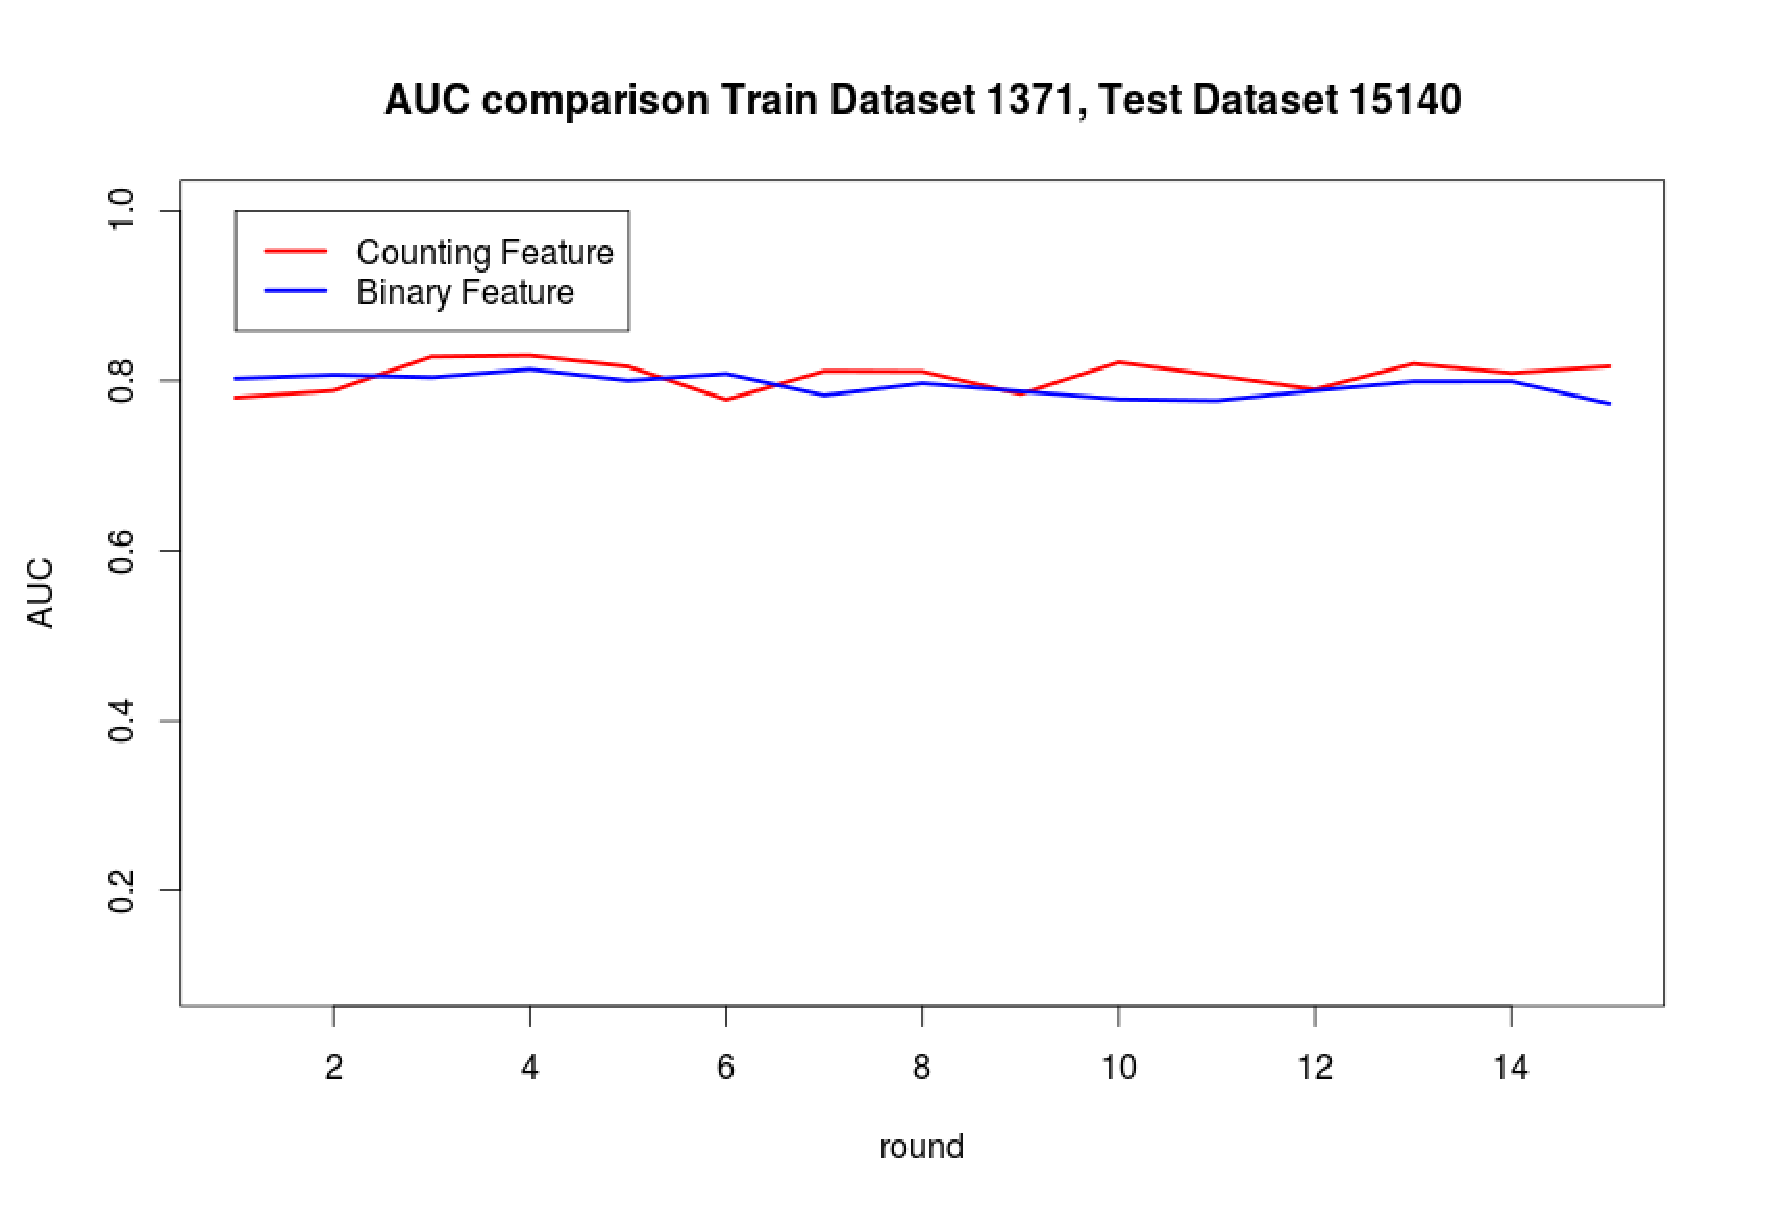
\includegraphics[width=\columnwidth]{1371_15140.eps}
\caption{Training Dataset  (1371), Test Dataset  (15140)}
\label{fig:fig7}
\end{figure}

Experiment 3.3: Training Dataset  (1371), Test Dataset  (12482) in Figure~\ref{fig:fig8}.:
\begin{figure}[h]
\centering
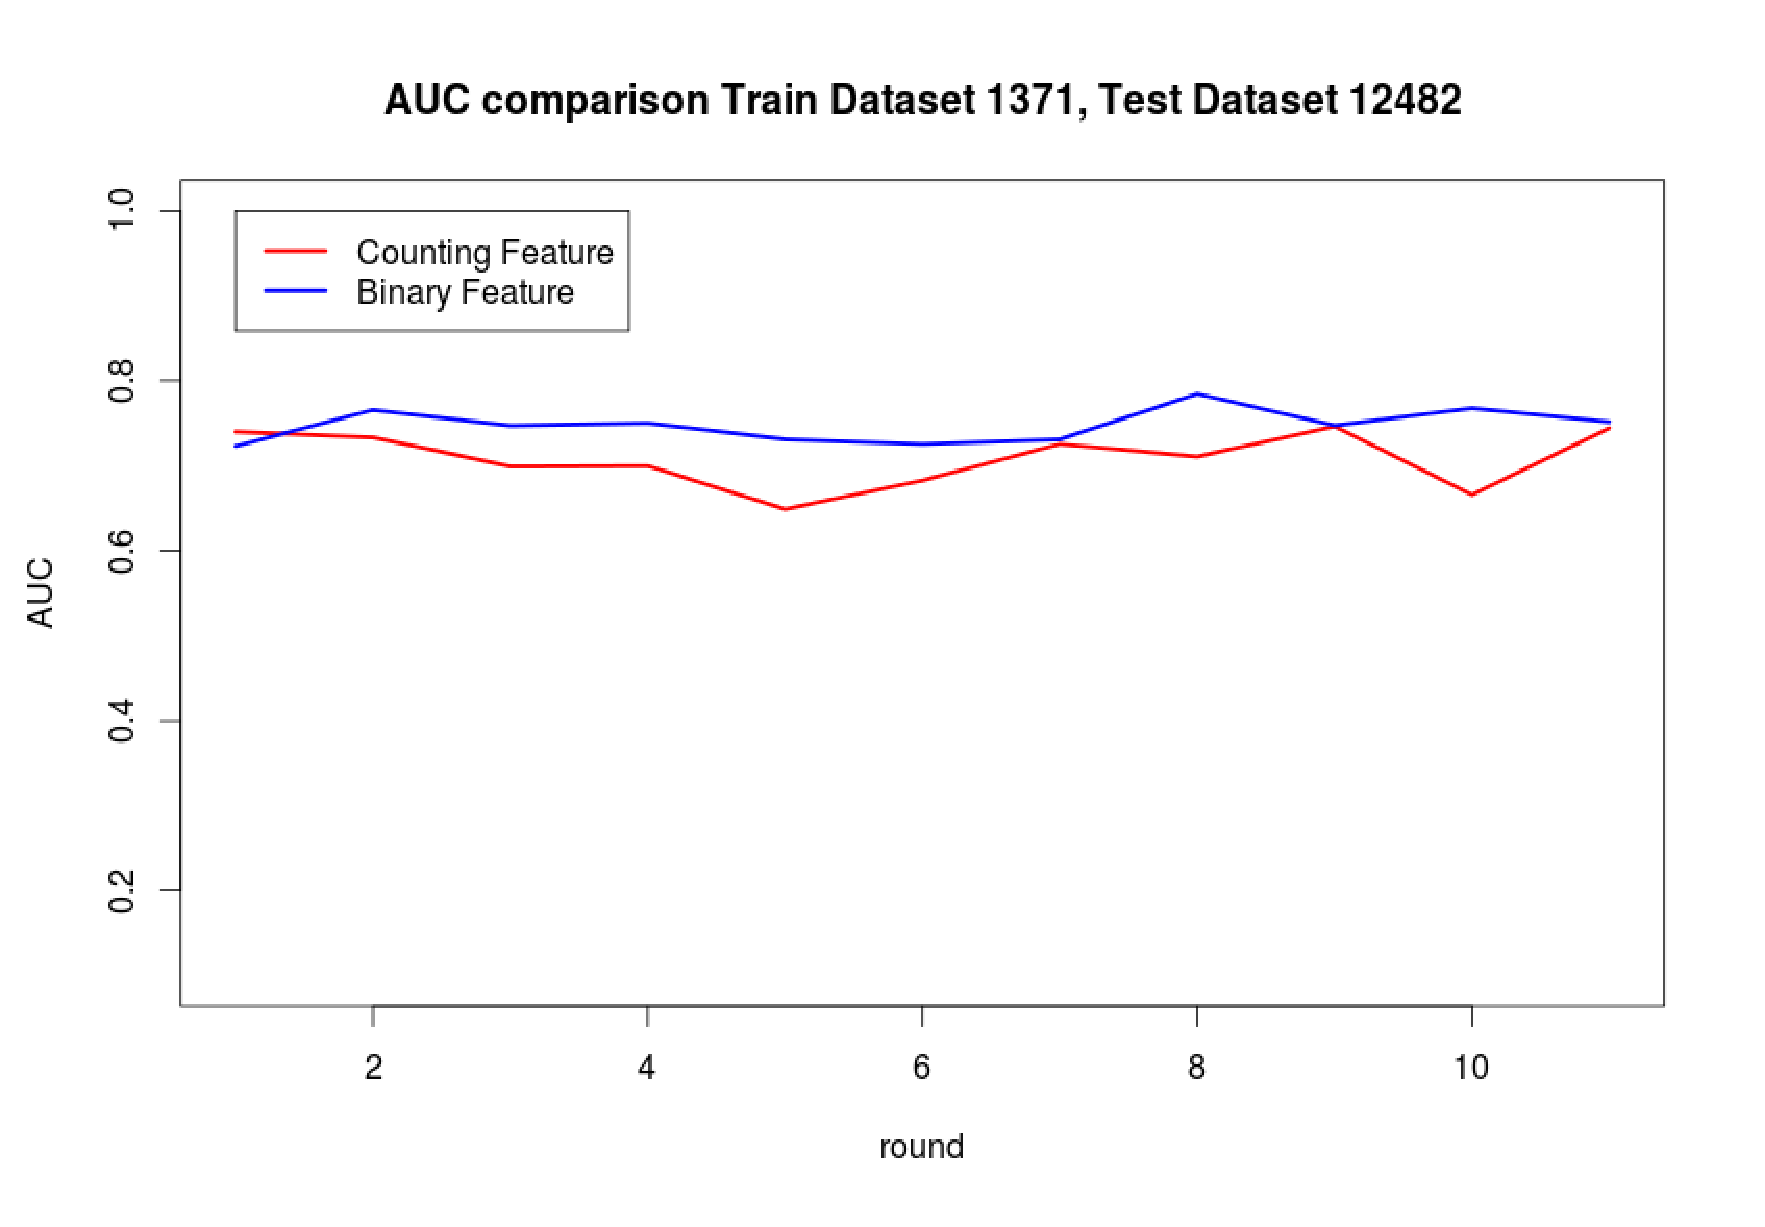
\includegraphics[width=\columnwidth]{1371_12482.eps}
\caption{Training Dataset  (1371), Test Dataset  (12482)}
\label{fig:fig8}
\end{figure}

Experiment 4.1: Training Dataset  (12482), Test Dataset  (20762) in Figure~\ref{fig:fig9}.:
\begin{figure}[h]
\centering
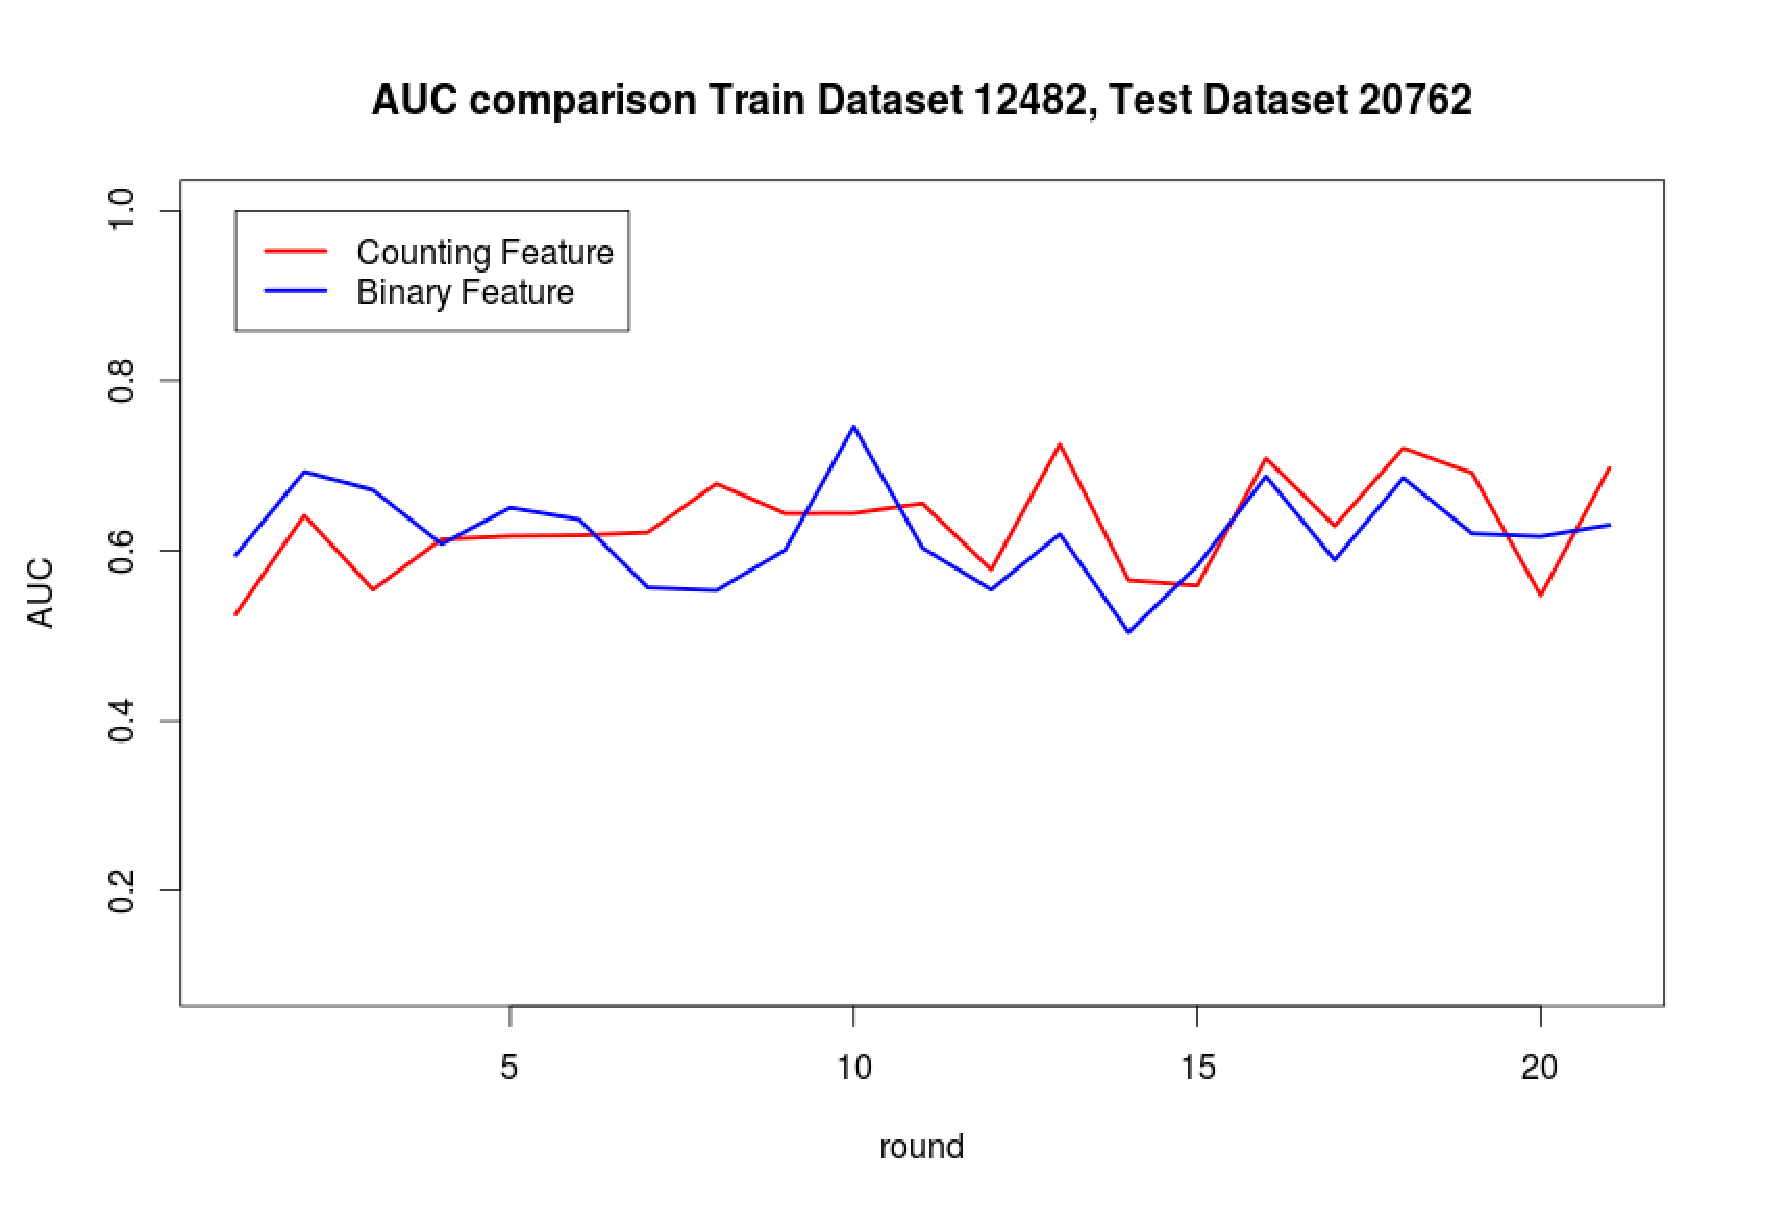
\includegraphics[width=\columnwidth]{12482_20762.eps}
\caption{Training Dataset  (12482), Test Dataset  (20762)}
\label{fig:fig9}
\end{figure}

Experiment 4.2: Training Dataset  (12482), Test Dataset  (1371) in Figure~\ref{fig:fig10}.:
\begin{figure}[h]
\centering
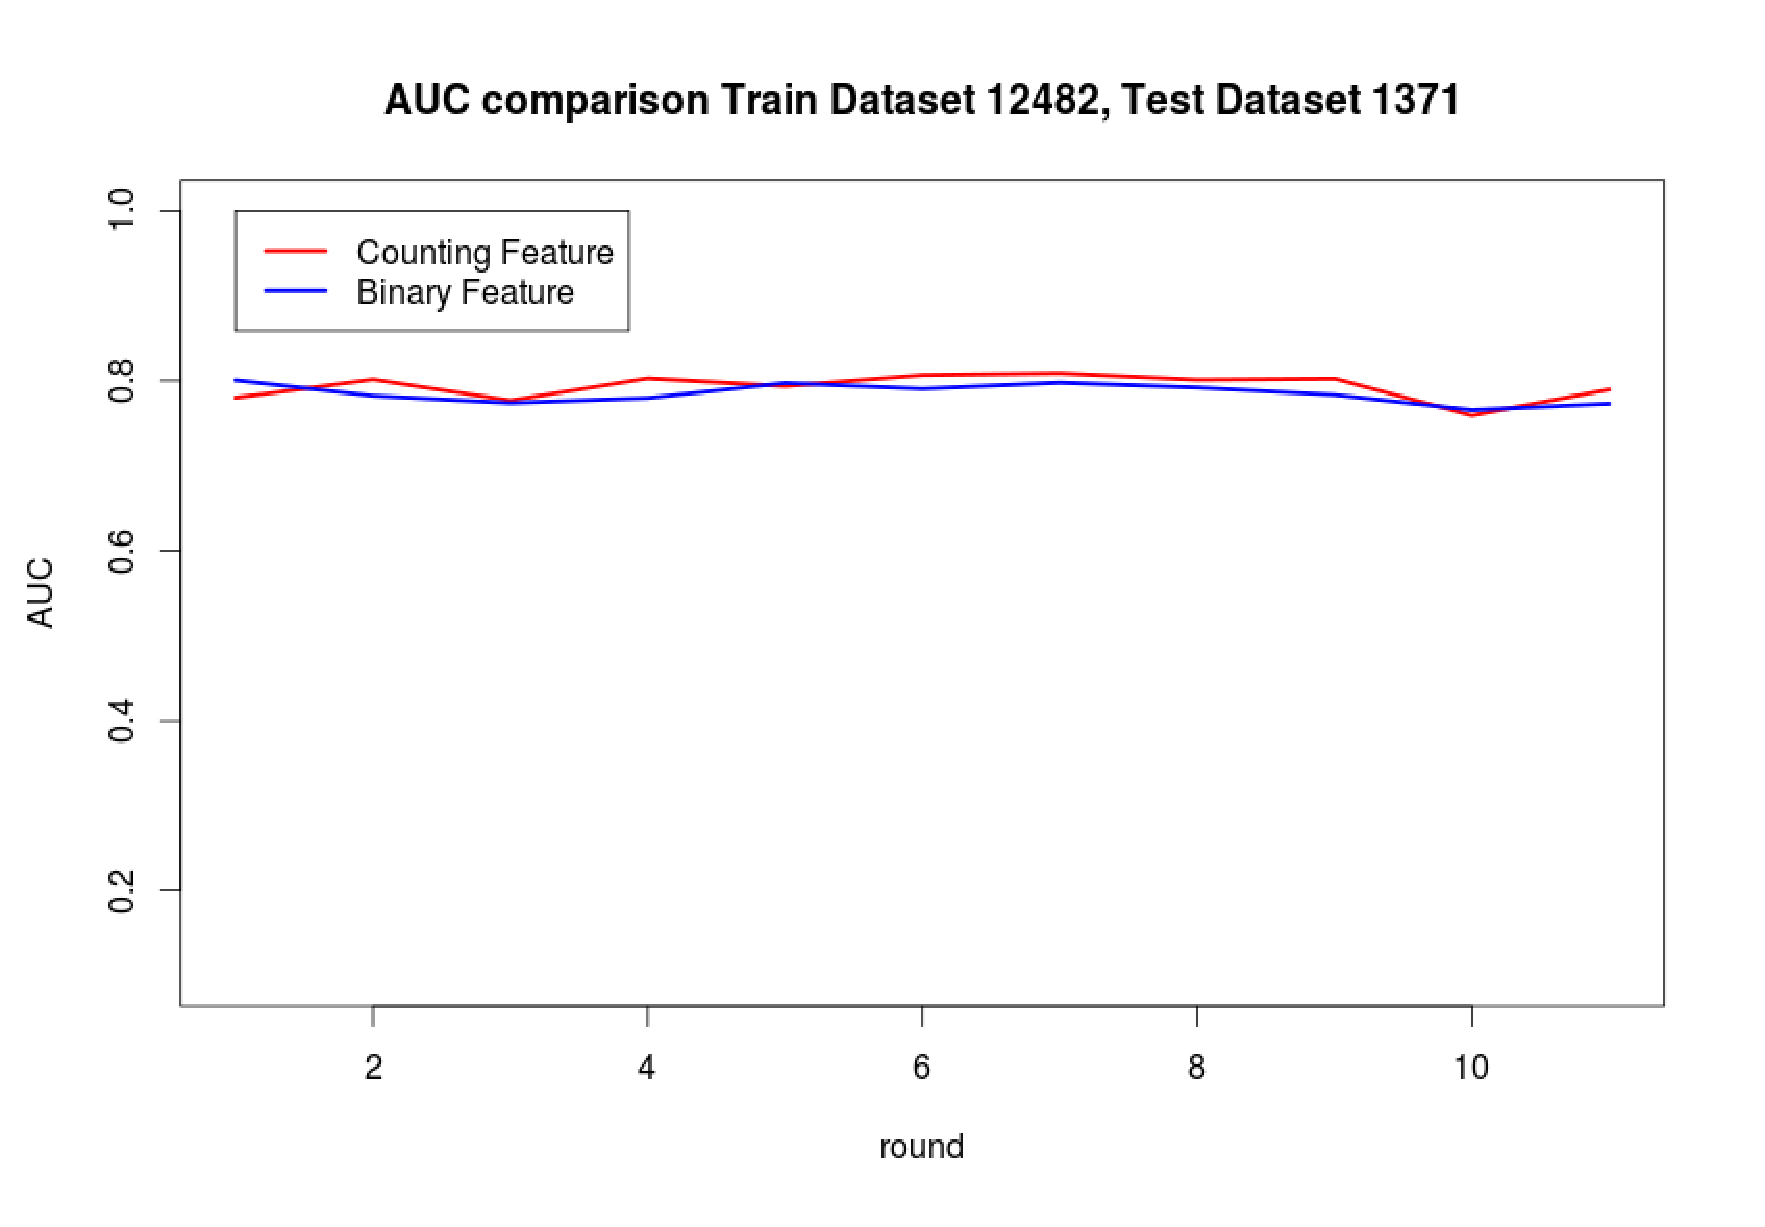
\includegraphics[width=\columnwidth]{12482_1371.eps}
\caption{Training Dataset  (12482), Test Dataset  (1371)}
\label{fig:fig10}
\end{figure}

Experiment 4.2: Training Dataset  (12482), Test Dataset  (15140) in Figure~\ref{fig:fig11}.:
\begin{figure}[h]
\centering
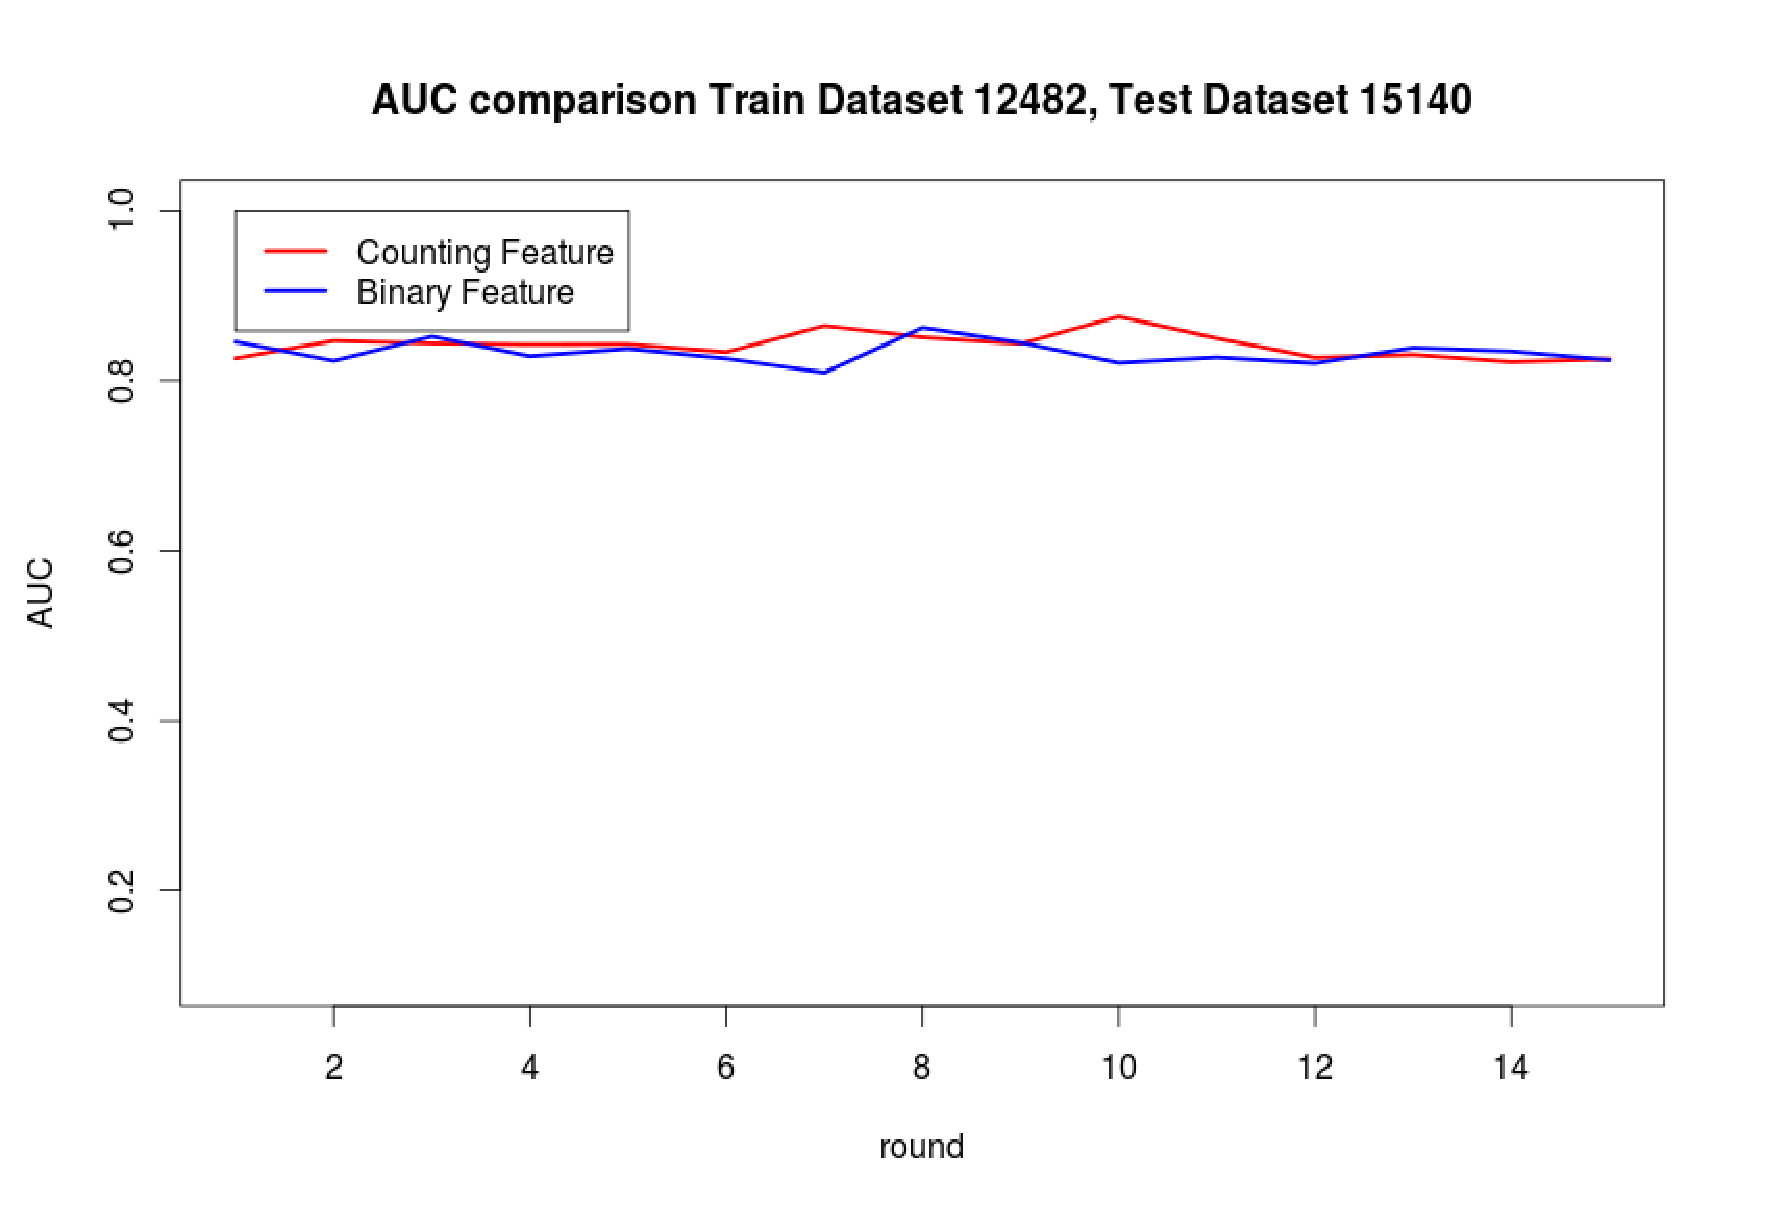
\includegraphics[width=\columnwidth]{12482_15140.eps}
\caption{Training Dataset  (12482), Test Dataset  (15140)}
\label{fig:fig11}
\end{figure}

\fi





\section{Conclusions}
 
%\end{document}  % This is where a 'short' article might terminate

%ACKNOWLEDGMENTS are optional
\section{Acknowledgments}




%
% The following two commands are all you need in the
% initial runs of your .tex file to
% produce the bibliography for the citations in your paper.
\bibliographystyle{unsrt}
\bibliography{sigproc}
% You must have a proper ".bib" file
%  and remember to run:
% latex bibtex latex latex
% to resolve all references
%
% ACM needs 'a single self-contained file'!
%
%APPENDICES are optional
%\balancecolumns

\end{document}
 